\documentclass[12pt, a4paper, oneside]{book}


%------------------------
% IMPORT PACKAGES
%-----------------------
\usepackage{amsthm}
\usepackage{mathtools}
\usepackage{algpseudocode}
\usepackage[chapter]{algorithm}
\usepackage{amssymb}
\usepackage{graphicx}
\usepackage{caption}
\usepackage{fancyvrb}
\usepackage{array}
\usepackage[acronym,toc,nohypertypes={acronym,notation},nonumberlist,automake]{glossaries}
\usepackage{hyperref}
\usepackage{epigraph}

%% remark theoremstyle
%\newtheoremstyle{break}
%{\topsep}{\topsep}%
%{\itshape}{}%
%{\bfseries}{}%
%{\newline}{}%
%\theoremstyle{break}
%\newtheorem{remark}{Remark}[section]

% problem theoremstyle
%\newtheoremstyle{problemstyle}  % <name>
%{10pt}  % <space above>
%{10pt}  % <space below>
%{\normalfont} % <body font>
%{}  % <indent amount}
%{\bfseries\itshape} % <theorem head font>
%{\normalfont\bfseries:} % <punctuation after theorem head>
%{.5em} % <space after theorem head>
%{} % <theorem head spec (can be left empty, meaning `normal')>
%\theoremstyle{problemstyle}
%\newtheorem{problem}{Problem}[section] % Comment out [section] toremove section number dependence
%\newtheorem{definition}{Definition}[section]
%\newtheorem{theorem}{Theorem}[section]
%\newtheorem{proposition}{Proposition}[section]
%\newtheorem{remark}{Remark}[section]
%\newtheorem{lemma}{Lemma}[section]
% create command for variance in math mode
%\newcommand{\Var}[1]{\operatorname{Var}\left[#1\right]}
\newtheorem{mydef}{Definition}[section]
\newtheorem{myexample}{Example}[section]
\newtheorem{myprop}{Proposition}[section]

\renewcommand\textflush{flushright}
\setlength\epigraphwidth{.6\textwidth}

\makeglossaries



\newacronym{GH}{GH}{Generalized Hyperbolic}
\newacronym{ED}{ED}{Event-Driven}



\begin{document}


%----------------------------------------------------------------------------------------
% COVER PAGE
%----------------------------------------------------------------------------------------
\pagestyle{empty}
\begin{titlepage}

	\begin{center}
		\normalsize 
			\textsc{Politecnico di Milano}\\
			Scuola di Ingegneria Industriale e dell'Informazione\\
      		Corso di Laurea Magistrale in Ingegneria Matematica\\
	\end{center}
	\vspace{.6cm}
	
	\begin{figure}[htpb]
		\centering
		
\includegraphics[width=4cm]{Cover/polimi}
	\end{figure}
	\vspace{.6cm}
	
	\begin{center}
		\LARGE
			\textsc{\textit{sign-to-contract}: how to achieve trustless digital timestamping with zero marginal cost}
	\end{center}
	\vspace{1.6cm}

	\begin{flushleft}
		\large
		\begin{tabular}{ll}
		Relatori:    & Prof. Daniele MARAZZINA      \\
		             & Prof. Ferdinando AMETRANO
		\end{tabular}
		\vspace{1cm}
	\end{flushleft}
	
	\begin{flushright}
		\large
		Tesi di Laurea di:\\
		Leonardo COMANDINI\\
		Matr. 863940\\		
	\end{flushright}
	
	\vspace*{\fill}
	\begin{center}
		Anno Accademico 2017-2018
	\end{center}
	
\end{titlepage}


%----------------------------------------------------------------------------------------
% ABSTRACT
%---------------------------------------------------------------------------------------

%% Set page numbers of the introduction to roman  
\frontmatter
\pagestyle{plain}
%\chapter{Abstract}
\label{chpr:abstract}

Proving that data existed prior to a certain times is helpful in several situation.
Thanks to systems achieving distributed consensus without relying of a trusted third party, like Bitcoin, it is possible to enhance the security of such timestamps.
OpenTimestamps is a protocol defining a standard for creating timestamps and, in addition, it provides scalability solutions.
Currently an improvement concerning elliptic curve commitments has been proposed. 
We aim to give a exahustive overview upon this new scheme, its implications and motivations, culminating in the development of a real world application.



%\cleardoublepage
\vspace*{\fill}
\epigraph{\textit{Sed quis custodiet ipsos Custodes?}\\But who will guard the guards themselves?}{Juvenal, c. 100 A.D.}
\vspace*{\fill}


%----------------------------------------------------------------------------------------
%	LIST OF CONTENTS/FIGURES/TABLES PAGES
%----------------------------------------------------------------------------------------

\tableofcontents
\listoftables
\addcontentsline{toc}{chapter}{List of Tables}
\listoffigures
\addcontentsline{toc}{chapter}{List of Figures}
\listofalgorithms
\addcontentsline{toc}{chapter}{List of Algorithms}
\printglossaries

\chapter{Abstract}
\label{chpr:abstract}

Proving that data existed prior to a certain times is helpful in several situation.
Thanks to systems achieving distributed consensus without relying of a trusted third party, like Bitcoin, it is possible to enhance the security of such timestamps.
OpenTimestamps is a protocol defining a standard for creating timestamps and, in addition, it provides scalability solutions.
Currently an improvement concerning elliptic curve commitments has been proposed. 
We aim to give a exahustive overview upon this new scheme, its implications and motivations, culminating in the development of a real world application.


\chapter{Acknowledgements}
\label{chpr:acknowledgement}

I would first like to thank my thesis advisor Prof. Marazzina for the always prompt help in writing the research.
Then I would like to thank Prof. Ametrano, who initially unveiled me the true nature of Bitcoin as a tool enhancing freedom, successively assisted me in my learning growth, ultimately he directed me in my research, advicing me when facing doubts and putting me back on track when I needed. 

Next I would like to acknowledge the experts whose work his the skeleton of the thesis, Peter Todd and Andrew Poelstra.
Todd is the first contributor to OpenTimestamps, his code and publications have been the essential landmark which inspired almost the whole research.
Poelstra is the author of the code extension that enables the technique examined in the research.

Furthermore I would like to thank the community behind Milano Bitcoin meetups, they give me the chance to meet experts and enthusiastic people, it motivated me to deepen my studies and contributed to improve my education in the subject.

Finally, I would also like to thank Eternity Wall team, specially Riccardo Casatta, Valerio Vaccaro and Luca Vaccaro.
Eternity Wall, leading company in the sector, hosted me for an internship during which the research was written, 
their mentorship has been indispensable to achieve the results composing this work.
They patiently counseled me in each step I had to take, teaching me the correct approach to tackle and solve specific technical problems in a professional manner. 
With extreme and consistent availability, they deeply involved me in the subject, sparking in me profound motivations.

%----------------------------------------------------------------------------------------
%	THESIS CONTENT - CHAPTERS
%----------------------------------------------------------------------------------------

\mainmatter

\chapter{Introduction}
\label{chpr:intro}
Associate dates with events is the essential medium to write history. 
In the distant past it was appanage of a restricted elite of powerful individuals, with the evolution and progress of society, the amount people able to write their own history has increased.
This lead to the emergence of different versions but, after all, it is not a crucial concern, as several human constructions, history can be a distortion of reality.
Converge to a single version is a tough matter, yet it is grounded to the ability of everyone to write their own history.
Preclude to some individuals the possibility to state and record their viewpoint may compromise incontrovertibly the bearing between history and reality.
In this work we focus on the primary obstacle: record arbitrary events.

Using proper semantics an event is mapped into data, which are embedded in an item suitable for storing and sharing, finally on the resulting object is attached a date. 
Each step can be performed in a variety of manners and each particular problem has its own optimal choices to fulfil at best the given requirements. 
In this work we assume the meaning of the data is given and we refer to the procedure of binding a date to data as timestamping. 
We focus on weaknesses and strengths of every choice, starting from physical to digital timestamping, posing particular emphasis on the trust issue.
If a third party is placing the date on the item containing the data, it may behave maliciously, among the things, compromising the data or setting a wrong date. This issue can be addressed by properly utilizing technologies achieving distributed consensus, like Bitcoin.
Such accomplishment let anyone write its own version of the events, oppressed people are given the possibility to record what they witness even in hostile environments, reducing powers and responsibilities of central authorities.

The actual implementation to make this viable and accessible on large scale presented tough technical steps. 
It resulted in the formation of an open protocol defining a standard and best practices \cite{OTSWeb} that are currently emerging as a new praxis to integrate in other systems to enhance security. 
The protocol is among the first and the few non-financial blockchain-related working applications \cite{ESMAresponse}.

Our contribution starts with a deep investigation of an improvement proposal \cite{PoePR, PoeIs} to the standard that yields to the chance to include a timestamp inside a bitcoin transaction without increasing its size and hence its cost. 
We aim to provide guidelines to properly understand what's behind this technique and the implications it carries.
Finally we present a practical implementation we developed of this new feature: an integration to a popular bitcoin open source wallet that allows users to create timestamps within transactions with no additional charge. 

\section{Structure}
In this work we aim to describe exhaustively foundations, benefits and issues of arising from the new proposed technique. 
It requires to traverse different subjects, mainly cryptography, computer science and distributed systems.
In this section we outline the path we are going to undertake.

In Chapter \ref{chpr:timestamping} we define what a timestamp is and we exploit the essential characteristics of its components: operations and attestations.

In Chapter \ref{chpr:trustless}, after a brief introduction on what Bitcoin is, we show how it can be used to achieve digital timestamping without relying on trusted third parties.

In Chapter \ref{chpr:state-of-art}, we show the state of the art of trustless digital timestamping, with the open source project OpenTimestamps. 
We provide a description of the standard it defines and the solution to address scalability issues.

In Chapter \ref{chpr:ec-commitments} we plunge into the core of the work, analysing the technique of elliptic curve commitment, with main focus on timestamping applications, particularly \textit{sign-to-contract}.

In Chapter \ref{chpr:s2c} we highlight the practical implications of \textit{sign-to-contract}, both benefits and issues. Finally we show a plugin for a popular open source wallet that implements the technique described.

To conclude, in Chapter \ref{chpr:conclusions}, we summarize what has been discussed and draw attention to which future works can start from the point reached.

\chapter{Timestamping}
\label{chpr:timestamping}
Placing a certain date on some data is surprisingly useful \cite{Haber91howto, Bayer93improvingthe, Massias99designof, OTSannouncment}.
An inventor who had a patentable idea or a scientist who came to a relevant conclusion may want to create a verifiable proof that at a certain moment they discovered something. This can help them to protect their intellectual property, proving others their precedence over competing claims.
In a communication protocol having the possibility to attach a certain time to messages can improve the security of the transmission. However it is often difficult to come to an agreement of which is the correct time to use, so different security models yield to different practical schemes.
When storing documents in a third party cloud server, it could behave maliciously, for instance modifying their contents. Placing a certain and tamper resistant date on a document will make harder for the server provider to corrupt that file: the attacker should also be able to falsify the certificate stating the date. 

Other practical applications of this technique are possible, however to have a complete understanding of the subject it is important to figure out which are its limits and which are the right choices to take to correctly put the concepts into practice. So we need to be a little more formal,
\begin{mydef}
	A timestamp is a proof that some data $d$ existed prior to time $t$.
\end{mydef}
To create such proof $d$ has to cause an event that could not have been generated without the existence of $d$. Such event it is binded to time $t$ and can be observed by others, we call its record \textit{time attestation}. So a proof consists in the data $d$, the set of \textit{operations} that were applied to cause the event and the time attestation.

Proofs are useful if they are able to convince the verifiers. He must be able to check the correctness of the operations and must retain trustworthy the time attestation. Depending on the problem in exam one should properly choose which operations and attestations to use. 

Let's consider the case of a sent letter. The data $d$ is the content of the letter, which caused the palpable letter: if $d$ were different the letter would be different. When the letter went through the post office a postmark with the date $t$ was stamped on the letter, the postmark is the time attestation. If the post officer is trustworthy, a verifier who examine the letter may be convinced that the content of the letter existed prior to the time stated in the postmark. However a good counterfeiter could change the content of the letter or falsify the postmark placing a false date, thus for some cases such proof would not be appropriate.

In the case of a digital document new problems arises: it is not necessary to be a good counterfeiter to falsify a document without leaving any kind of tamper evidence, thus new solutions must be adopted. A timestamp for the data $d$ should guarantee that if even only a single bit of $d$ is modified the timestamp proof becomes invalid. To solve this problem cryptography tools are used \cite{Haber97securenames}. Digital data can also be shared easily and with little costs, this is among the features that enables the possibility to achieve distributed and decentralized consensus. Such an achievement would give user the chance to timestamp without any trust in a third party.

Resuming, at a certain moment $t_e$ some data $d$ exists, then at $t_c$ someone (or something) will have the necessity to prove the existence of $d$, so he implements the timestamp \textit{creation procedure} that results in a proof stating that $d$ existed priort to time $t$. Consequently at time $t_v$ a challenger implements the \textit{verification procedure} that ends in a binary result: true if he retains the proof correct, false otherwise. Naturally we have $t_e<t_c<t<t_v$.

To avoid common misunderstandings, it is important to clarify what a timestamp does not proves. The time $t$ is the first moment when $d$ went to existence, the creation procedure is not instantaneous and of course if the proof for $(d,t)$ is true then there exists a proof for $(d,t')$ which holds true for all $t'>t$. A timestamp is not necessarily linked to its creator and moreover it doesn't prove that who owns the timestamp (it can be owned by multiple entities) is the creator of the data $d$: it just proves that someone knew $d$. If an inventor comes up with a timestamp stating that he had a particularly smart idea prior to time $t$, it does not mean that he was the first one to have such idea, in fact he could have simply overheard the idea from a colleague and afterwards timestamped it. A timestamp does not prove that data $d' \neq d$ does not exist. Imagine someone stating that he knew the result of the elections prior to vote, he provides a timestamp and claims that it proves he predicted the correct result. However he could be a imposter: he may had timestamped several different results and once he saw how the vote count ended he will provide only the proof which make him look as a visionary.
Although these limitations being able to timestamp is still useful. If stronger proofs are needed the used system must be endowed with other tools that actually provides what is asked. 

In the following sections we analyse the two ingredients of timestamp proof: operations and attestations.

\section{Commitment Operations}

The operations that compose a timestamp proof should be defined in a precise way, a verifier will check their correctness when evaluating the proof. An useful operation binds the data in a way that it is hard or impossible to modify the data after the creation of the timestamp. Being more general, such an operation commits the input to the output: the input cannot be changed without changing the output. The result of the operation is a commitment to the input, in the sense that it was caused by the input or, in other words, the input precede in time the output.
For instance in the case of a sent letter, the input is the content of the letter, the piece of paper that is sent is the output and physically writing the letter is the operation that commits the input to the output. We can say that a letter is physical commitment to its content. If one wants to modify the content of the letter ex post it will change the letter itself. However, tamper evidence could be extremely hard to spot.

Digital document are easier to tamper, but they could be defined in a more precise way, representing each document with bits. To take full advantage of this we need a formal definition,
\begin{mydef}
	A function $C:X \rightarrow Y$ is a commitment operation if given $x_1 \in X$ it is not feasible to compute $x_2 \in X$ s.t. $x_1 \neq x_2, C(x_1)=C(x_2)$.
\end{mydef}
The property required is sometimes referred as second pre-image resistance. For practical purposes $X$, $Y$ can be thought as bit string spaces, its element can be seen as bit strings or another of their representations, for instance in hexadecimal digits or using a conventional encoding.
The simplest examples are the append and prepend operations:

\begin{myexample}
	\textquotedblleft hello\textquotedblright $\xrightarrow{\text{append(\textquotedblleft world\textquotedblright)}}$ \textquotedblleft helloworld\textquotedblright
\end{myexample}
It is impossible to change the input without changing the output: the output contains the input itself. In this example the function is a unary operation, since it takes only one input, however commitment operation may have more than one input:
\begin{myexample}
	\textquotedblleft world\textquotedblright, \textquotedblleft hello\textquotedblright $\xrightarrow{\text{prepend()}}$ \textquotedblleft helloworld\textquotedblright
\end{myexample}
Append and prepend have two problems: they reveal everything about the inputs and the size of the output is always greater than the size of the inputs. 

Hiding the input of a commitment is often useful. For instance Robert Hooke \cite{Petroski96invention} in 1676 had formulated the spring law that will take his name. He wanted to prove that he knew that without revealing the law itself, so he published the latin anagram \textquotedblleft ceiiinosssttuv\textquotedblright. Later in 1678 he revealed the solution, \textquotedblleft ut tensio, sic vis\textquotedblright (\textquotedblleft as the extension, so the force\textquotedblright). However the anagram is not an optimal commitment operation: \textquotedblleft ut vis, sic tensio\textquotedblright is a solution too. For that time it was an acceptable solution, the verification procedure had minimal requirements and there was no real incentive in lying. Nowadays better solutions are available, hence using an anagram will make the verifier suspicious.

To address this problems cryptographic hash functions are used. Hash functions maps bit strings of arbitrary finite length into bit strings of fixed length \cite{Damgard:1989:DPH:118209.118248}. 
\begin{mydef}
	$h : \{ 0, 1 \} ^* \rightarrow \{ 0, 1 \} ^n $ is a hash function if it is computable in polynomial time in the length of the input.
\end{mydef}
We will refer at the input of such functions as preimage, and the output as hash value. The codomain is strictly contained in the domain hence the presence of collisions (pairs of inputs with identical outputs) is unavoidable. 
To give to these functions a practical use some of the following properties are required
\begin{mydef}
	\label{hash-prop}
	Let $h$ be a hash function, the following properties may hold:
	\begin{itemize}
		\item preimage resistance: given $h(x)$ it is not feasible to compute $x$;
		\item second-preimage resistance: given $x$ it is not feasible to compute $y$ s.t. $x \neq y$, $h(x)=h(y)$;
		\item collision resistance: it is not feasible to find $x, y$ s.t. $x \neq y$, $h(x)=h(y)$.
	\end{itemize}
\end{mydef}

A preimage resistant hash function hides the inputs, this property is sometimes referred as one-wayness.
A second-preimage resistant hash function is also a commitment operation, in addition it hides the input and create a fixed size fingerprint. A huge file can be mapped into a short bit string which is a commitment to it.
Collision resistance, although is a nice to have, is not necessary for timestamping purposes: when a collision ($x \neq y$ s.t $h(x)=h(y)$) is found, $x$ and $y$ are found at the same time \cite{SHA1}.

Such properties depend on the dimension of the codomain, which is given by the parameter $n$, precisely $2^n$. If it is too low it will be easy to produce examples that invalidates the properties, if it is too high the hash function is not a good tool for reducing the size of the input. A good compromise has to be found, it should be based on the current state of the art of cryptanalysis and computer science. However what is considered acceptable during a period may not be accepted in a subsequent one, in fact if new techniques that break an hash function are discovered, then its use will be considered insecure.
Several hashing functions has been proposed, we show a couple of examples:
\begin{myexample}
	SHA1 (Secure Hashing Algorithm) was designed by the National Security Agency (NSA), and released in 1995. It maps bit strings to a 160 bit space, it was considered preimage, second-preimage and collision resistant. In 2005 cryptanalysts discover a procedure to find collisions, hence it was declared insecure. However only collision resistance was broken, thus, for it can still be used for timestamping purposes.
	\begin{verbatim}
	SHA1(b'Hello World!\n') = a0b65939670bc2c010f4d5d6a0b3e4e4590fb
	                          92b
	SHA1(b'Hello World\n')  = 648a6a6ffffdaa0badb23b8baf90b6168dd16
	                          b3a
	\end{verbatim}
\end{myexample}

\begin{myexample}
	SHA256 belongs to the family SHA2, the generation of hash functions following SHA1. It has a outputs of 256 bit length and, at the moment, it is considered to satisy all the properties in Definition \ref{hash-prop}.
	Several systems are built upon this assumption. 
	In addition, as other hash functions, SHA256 could be modeled as a random oracle, a fixed input will provide always the same output, since hash functions are deterministic, but the outputs corresponding to new inputs will give a results, that for someone with a reasonable amount of computing power, are indistinguishable from a uniform distribution. 
	Note how a little change in the input produces outputs very dissimilar in both hash functions, this feature helps to spot alterations in the inputs.
	\begin{verbatim}
	SHA256(b'Hello World!\n') = 03ba204e50d126e4674c005e04d82e84c21
	                            366780af1f43bd54a37816b6ab340
	SHA256(b'Hello World\n')  = d2a84f4b8b650937ec8f73cd8be2c74add5
	                            a911ba64df27458ed8229da804a26
	\end{verbatim}
	Since SHA256 is available, the use of SHA1 should be avoided unless there is a particular motivation. 
\end{myexample}

More complex commitment operations are possible.
But they should be used only if there are some valid and shared motivations. Finding a badly motivated commitment operation in a proof will make verifiers suspicious.

Combining the examples we saw it is possible to implement a data structure that is useful to embed several commitments into a single hash value, 
this structure is called \textit{Merkle tree} [Mer]. Let $h$ be a second-preimage resistant hash function, start from $k$ data to timestamp $\{d_i\}_{i=1}^k$, called \textit{leaves}, compute their hash values $\{h(d_i)\}_{i=1}^k=\{h_i\}_{i=1}^n$. The first step combines the couples of adjacent values (if there is one) by concatenating ($||$) the two values and computing the hash value of the concatenation: $h(h_i||h_{i+1})$ $\forall i \in [1,k]$ odd. The following steps proceed in an analogous manner, but starting from the results computed at the step before as described in Algorithm \ref{alg:merkle-tree}. 

\begin{algorithm}
	\caption{Merkle tree construction}
	\label{alg:merkle-tree}
	\begin{algorithmic}[1]
		\Procedure{merklestep}{$\{h_i\}_{i=1}^k$}
		\State $S \gets \{\}$
		\For {$i\gets 1,k$ s.t. $i\equiv 1 (2)$}
		\State $S \gets S \cup \begin{cases} 
		h(h_i||h_{i+1}) & i \neq k \\ 
		h(h_i) & i=k           
		\end{cases}$
		\EndFor
		\State \textbf{return} $S$
		\EndProcedure
		\Statex
		\Procedure{merklelize}{$\{d_i\}_{i=1}^k$} \Comment{from the leaves to the Merkle tip}
		\State $S \gets \{\}$
		\For {$i\gets 1, k$}
		\State $S\gets S \cup h(d_i)$\Comment{hash the leaves}
		\EndFor
		\State $k\gets |S|$
		\While {$k \neq 1$}
		\State $S \gets$ \Call{merklestep}{S} \Comment{if necessary, store $S$}
		\State $k\gets |S|$
		\EndWhile
		\State \textbf{return} $S$ \Comment{Merkle tip}
		\EndProcedure
	\end{algorithmic}
\end{algorithm}

After at most $\lceil log(k) \rceil$ steps the algorithm ends and one hash value is returned, it is called \textit{Merkle tip} or \textit{Merkle root}. 
Thanks to reiteration of $h$ the tip is a commitment to all the leaves $\{d_i\}_{i=1}^k$, moreover to prove that a element $d_i$ is committed it is not necessary to know all tree, infact it's enough to show the \textit{Merkle path} starting from $d_i$ and ending in the tip. 
For instance referring to Figure \ref{fig:merkle-tree} the minimal requirement to show the commitment of $data3$ in $MT$ is the ordered sequence of operations to apply is:
\begin{verbatim}
h, append(h4), h, prepend(A), h, append(E), h
\end{verbatim}
Merkle trees can aggregate several commitments into one hash values, giving a scalability solution: the length of a single proof growth logarithmically with the number of leaves.

\begin{figure}
	\begin{center}
		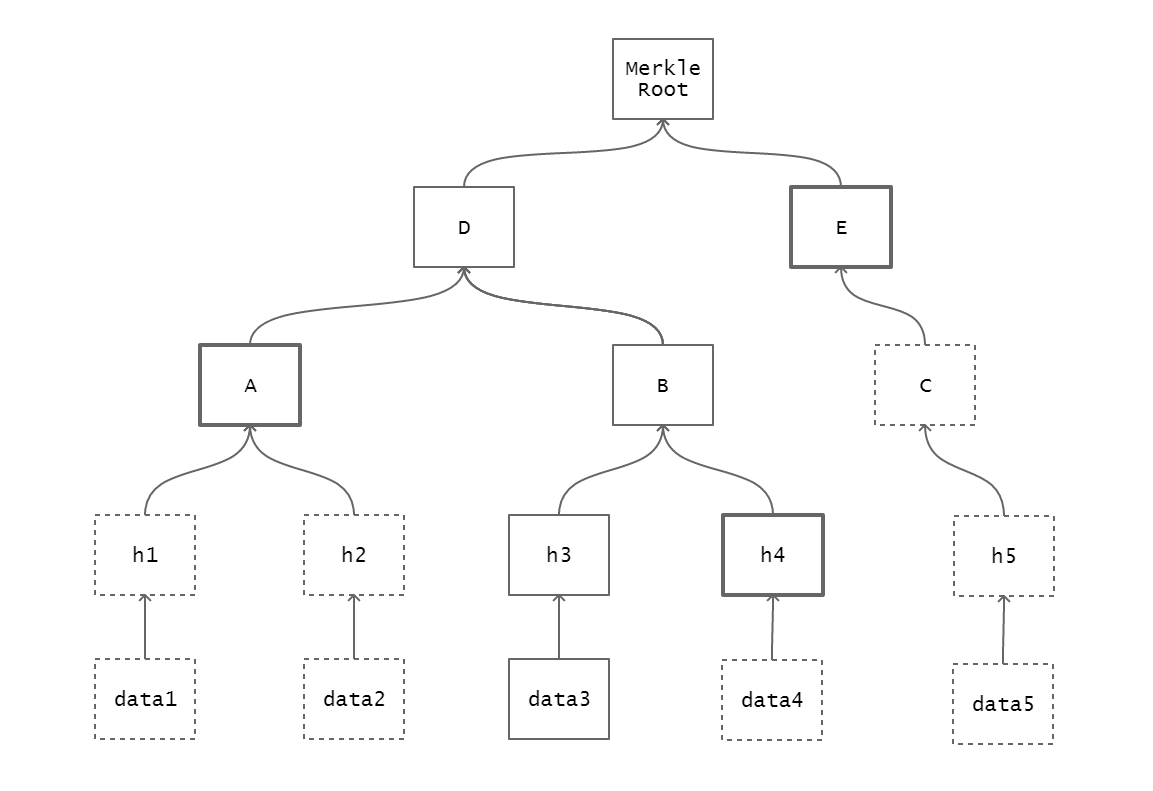
\includegraphics[width=\linewidth]{Images/merkle-tree.png}
		\caption[Merkle tree example]{Merkle tree example. the Merkle root is a commitment to the leaves $\{data_i\}_{i=1}^5$.}
		\label{fig:merkle-tree}
	\end{center}
\end{figure}

\section{Time Attestations}

Attestations are provided by a notary, which has the authority to state the time.
Notaries are sometimes referred as timestamp servers, who ask for creating or verifying a timestamp is referred as client.
A time attestation binds some data $d$ to the time $t$, $d$ could be directly the data to timestamp or a commitment to them. 

An attestation should be \textit{tamper resistant} or, even better, \textit{immutable}. Once created no one should be able to modify that, backdating the timestamp or changing the underlying data without making the attestation invalid.

In the case of a sent letter an important issue comes to the attention: the attestation (postmark) can be verified only if the letter is in our hands. This makes the task of a counterfeiter easier, few people will examine the postmark making the success of the attack more likely. A solution that mitigates this issue is \textit{widely publishing} the attestation, for instance inserting it in a newspaper. The attacker has an harder task, in most cases, to guarantee himself good chances of success he needs to modify several, or even all, attestations leading to a higher cost. Considering an attestation on a newspaper, an attacker could counterfeit only the exact copy the verifier is going to check. To prevent such situation the verifier should check multiple sources and should not expose any infomration on where he is retrieving the copies used to examine. Attestations should be \textit{easily accessible}, for instance a good solution is to publish them on the internet.

We call the service providing the attestations notary, it has the authority to state the time. To maintain such power it has to show itself as \textit{trustworthy}: it should place the correct time in the attestations, it should not trick the clients modifying the timestamp ex post and he should not collude with the creator of the timestamp to trick a verifier. Moreover a notary should be \textit{competent}: if it looses the information necessary to verify the timestamp its creator will be damaged.

A good notary does not make distinctions among clients or data to timestamps, in other words it does \textit{not censor}. An improvement would be if it is not aware of what it is timestamping, like the case of the commitments hiding their inputs, but even better if it is not aware of being used as a timestamp server, like the newspaper.

In the case of a sent letter, the notary is the post officer, he will place the postmark on the letter giving it a date. 
Clients must trust such notary, which in theory can place a wrong date $t'$ instead of $t$, creating a false timestamp (if $t'<t$) or a deliberate weaker proof (if $t'>t$). Alternately he can decide not to timestamp a letter or modifying its content before timestamping. In addition the resulting timestamp is unique, thus if it get damaged or lost the proof is gone forever.

A notary willing to show himself as more trustworthy can make its possibly dishonest behaviour harder to implement. A possible solution is to link all the timestamps so that changing one would implies changing all the subsequent ones. A timestamp proof $TS_i$ for the data $d_i$ at the time $t_i$ ($t_{i-1}<t_i<t_{i+1}$) would be something like:
\begin{equation}
	\label{singed-chain}
	\begin{cases}
		TS_0 =(d_0,t_0), \sigma_N((d_0,t_0)) & 
		\\
		TS_i =(d_i,t_i,TS_{i-1}, \sigma_N((d_i,t_i,TS_{i-1}))) & i = 1, ..., i_{max}		
	\end{cases}
\end{equation}
where $\sigma_N (x)$ is a commitment to the data $x$. Such commitment is created by the notary, who is (supposely) the only one who is able to apply $\sigma_N$. We call this function \textit{signature}, it can be physical (as a postmark) or digital (with a public key cryptosystem). The signature $\sigma_N$ is a commitment operation, so if $TS_{i}$ changes then $\sigma_N((d_{i+1},t_{i+1},TS_i))$ changes, thus $TS_{i+1}$ changes resulting in $TS_j$ changing for all $j>i$. Starting from the \textit{genesis timestamp} $TS_0$, the linked timestamps $\{ TS_{i} \}_{i=0}^{i_{max}}$ form a \textit{chain}. A trusted notary which implement this scheme will be preferred by honest clients. Depending on each particular problem the designer of the system has to properly choose how to collect the timestamp requests, how to commit them into the chain, the time frequency, the signature procedure, how to publish the chain and how to distribute the timestamp proof to the clients.

Even though linking the timestamps is a great improvement with respect to the previous schemes, having a trusted notary still involves some issues. The notary may loose what he needs for signing (e.g. stamp, private key); if an attacker can sign in the place of the notary, it will no longer be considered authoritative; if no one can sign the clients will be damaged. In addition the notary can create more than one chain starting from the same genesis timestamp, then he can use different chains for different clients. 
Anyhow nothing can guarantee that a trusted notary will behave honestly in the future, it can attack some clients in several ways and such bad behaviour can be hard to spot rapidly, a single client may realize that he has been tricked only when he needs the timestamp.

Trusted attestations has security issues hence, in some situations, they could be considered not enough appropriate, yet for years an efficient solution that does not involve a trusted third party was considered barely impossible. 
In 2008 Satoshi Nakamoto proposed \cite{Nakamoto_bitcoin:a} which described a system to transfer value from one party to another without relying on the presence of a central authority. The system can be also used to timestamp arbitrary data without trusting any notary.

\chapter{Trustless Timestamping}
\label{chpr:trustless}
Bitcoin enables timestamping in a trustless framework. 
To show this first we introduce what Bitcoin is and why it works, then we show two techniques to timestamp data using the protocol's digital coins.

As a premise it is important to highlight why and in which terms a trustless design is superior to a trusted one. 
Trusted schemes can be built upon trustless ones, but the other way around is not possible. 
Trustless systems have higher security but the mechanism sustaining it makes thing much more sophisticated, yielding to less accuracy and efficiency with respect to trusted ones.

\section{Bitcoin}
Bitcoin is an electronic payment system based on cryptography rather than trust. A \textit{coin} is defined as a chain of digital signatures. Each owner transfers the electronic coin to the next by digitally signing a hash of the previous \textit{transaction} and the public key of next owner (or a commitment to it).

Coins doesn't have to be managed individually, they can be combined and split in transactions containing multiple inputs and outputs. The last output appended to a coin is said unspent transaction output, UTXO.

However who receives a transaction cannot verify that who pays him did not \textit{double-spend} the coin. 
To prevent this behaviour it is needed a system to agree on a single history of the order in which the transactions were received. The proposed solution starts with a timestamp server: each timestamp it's a hash of a \textit{block} which contains a set of items and the previous timestamp (if there is one). The resulting data structure forms a chain, which is sometimes referred with the (at the moment of writing) overhyped term \textit{blockchain}. 
\begin{equation}
	TS_i =
	\begin{cases} 
		h(items_0) & i=0\\ 
		h(TS_{i-1} || items_i) & i=1, ..., i_{max} 
	\end{cases}
\end{equation}
To implement a \textit{distributed} version of a timestamp server it is used a \textit{proof-of-work} (PoW) system similar to Adam Back's Hashcash \cite{Back02hashcash-}. The proof-of-work consist in scanning for a value (called \textit{nonce}) to be included in the block that when hashed produces an hash value (interpreted as an integer) less then a given target $w$ as pointed in Definition \ref{pow}.

\begin{mydef}{\textit{proof-of-work}}
\label{pow}
\\
\textbf{Given}:
\begin{itemize}
	\item previous timestamp $TS_{i-1} \in \{0,1\}^n$
	\item items to timestamp $items^i \in \{0,1\}^*$
	\item target to beat $w>0$
\end{itemize}
\textbf{Find}:
\begin{itemize}
	\item $nonce \in \{0,1\}^*$ s.t. $h(TS_i || items_{i+1} || nonce) < w$
\end{itemize}
\end{mydef}

The proof of work is basically finding partial hash collisions for the leading zero bits. Hash functions such SHA256 are designed in a way that the fastest algorithm for computing partial collisions is brute force. Thus finding a solution to the challenge is computationally expensive, in other words finding a soltution proves that CPU time was consumed and energy was destroyed for that purpose.
 
If the hash function has a sufficiently large codomain, it can be, in practice, arbitrarily hard to find a solution. For instance consider SHA256, the codomain is $\{0,1\}^{256} \approx \mathbb{Z}_{2^{256}}$, assuming that its outputs have the same probabilities, the chance that a given $nonce$ has hash value less then the target is $\frac{w}{2^{256}}$.  
If $w=1$ the proof-of-work is finding a pre-image of 0 (with additional constraints) but that is not feasible thanks to its preimage resistance property. 
So the lower is $w$ the higher is the difficulty, tending towards an unfeasible problem as $w$ is closer to 1. 
Assuming that the computational power used is known, the target can be chosen so that expected time to find a solution matches a given value.

The proof-of-work is \textit{publicly auditable}: when a solution is found verifiers check its correctness computing a single hash and perform one comparison. If the verification is successful they are convinced that someone has done the work, without the need to know or trust him. In other words \textit{proof-of-work commits energy to data}.
This commitment takes the place of the signature in the linked timestamping scheme (\ref{singed-chain}), to extend the chain is not necessary to be able to sign as a notary, instead anyone running a particular software can try to solve the proof-of-work, who finds the solution will append it to the chain. 
\begin{equation}
\label{chain-nonce}
TS_i =   
\begin{cases} 
h(items_0) & i=0\\ 
 h(TS_{i-1}||items_i||nonce_i) & i=1, ..., i_{max} 
\end{cases}
\end{equation}

However the proof-of-work by itself does not prevent the double-spending problem, it makes computationally expensive to rewrite a chain, but alone it does not ensure that the chain is unique.

Bitcoin can be seen as a network, nodes are entities who run a software following a protocol. The network behaviour can be designed as follows:

\begin{algorithm}
	\caption{Bitcoin network behaviour}
	\begin{algorithmic}[1]
		\State New transactions are broadcast to all nodes.
		\State Each node collects new transactions into a block.
		\State Each node works on finding a difficult proof-of-work for its block.
		\State When a node finds a proof-of-work, it broadcasts the block to all nodes.
		\State Nodes accept the block only if all transactions in it are valid and not already spent.
		\State  Nodes express their acceptance of the block by working on creating the next block in the chain, using the hash of the accepted block as the previous hash. % previous timestamp?
	\end{algorithmic}
\end{algorithm}  

Honest nodes always consider the chain with the most proof-of-work to be the correct one and will keep working on extending it.
If two nodes find different versions of the next block simultaneously, the network will be split into two sets with different chains. 
The tie will be broken when the next solution is found: one chain will have more proof-of-work then the other, the nodes working on the other branch will switch to the longer one; this event is called \textit{reorg}. 
Reorgs greater than one block may happen, but with exponentially decreasing probabilities, given that the majority of the nodes does not collaborate to behave maliciously; for practical purposes a transaction is considered \textit{confirmed} after 6 blocks are appended to the block including the transaction.

By convention the first transaction in a block is a special transaction that starts a new coin owned by the creator of the block, called \textit{coinbase}.
It provides an \textit{incentive} to the nodes performing the proof-of-work and provides a way to initially distribute coins into circulation, since there is no central authority to issue them.
This minting procedure mimes gold extraction: instead of expending resources to add gold to circulation, in this case CPU time and energy is consumed to bring to light new coins. 
Actually nodes with few computational resources can decide that their chances to find a solution are too low for even trying, thus only some nodes will attempt to solve the proof-of-work, following the previous analogy they are called \textit{miners}.
The incentive can be also funded with \textit{transaction fees}, which are the difference between inputs and outputs amounts. Fees give a way for miners to prioritize transactions, higher fees will be preferred, they also provide an anti denial-of-service measure, for each spamming transaction the attacker has to spend a fee greater or equal then the some of the ones competing with it to get into a block.
The incentive may help encourage nodes to stay honest. 
A miner with enough computational power can defraud people by sending them coins and then rollback the transactions extending another chain not containing such transaction. 
However this undermine the system, people won't use it to send payments and the coins will loose their value, damaging its own wealth.
He ought to find more profitable to play by the rules, contributing to increase the security of transactions and, as a consequence, of the value of the coins.

If the majority of the miners does not collaborate to attack the network, the nodes reach consensus over the state coins. The chain with the most work contains the history of all transactions, giving all the information to retrieve which are the coins that have not been spent, the UTXO set, and to check that no extra coin was created outside the network minting rules.
 
The result is surprising, in the network each node has an arbitrary behaviour, it may go offline, send false message, lie and attack other nodes. A node with this behaviour is called Byzantine \cite{Wattenhofer:2016:SB:3002702}, otherwise is called honest; 
finding consensus in a network with Byzantine nodes is called Byzantine agreement.
Bitcoin combines cryptography, proof-of-work and a economic incentive to create a system that comes to a Byzantine agreement. 
The key aspect is that the economic incentive is given with the same digital asset the the system is securing; if the economic incentive was unrelated to the system miners may start to behave maliciously.
Although is often misunderstood, the technology underlying Bitcoin is not suitable to come to a Byzantine agreement on arbitrary subjects aside from the history of the coins only. It is possible to build a system upon Bitcoin but it would require another layer of consensus.

Nodes in the network must agree on a common set of rules, including which is \textit{genesis block} and whether a transaction is valid. The rules define the consensus, which in turn defines the chain. If a set of nodes follow different consensus rules the network will split in two networks with different chains. If the two networks share the genesis block and a part of the chain, then it is called a \textit{fork}. We call the set of consensus rules followed by the Bitcoin network \textit{Nakamoto consensus}, however to properly address fork issues a further specification may be necessary. 

The size of the block may be excessive for some purposes, to save space the transactions are packed in Merkle tree, which is committed along with other items is committed in the \textit{block header} which is described in Table \ref{tab:block-header} taken from \cite{BitcoinDev}.

\begin{table}
\begin{center}
\begin{tabular}{|p{5cm}|p{5cm}|}
	\hline
	\textbf{Name} (bytes) & \textbf{Description} \\ \hline
	version (4) & The block version number indicates which set of block validation rules to follow \\ \hline
	previous block header hash (32) & A SHA256(SHA256()) hash of the previous block’s header \\ \hline
	merkle root hash (32) & Merkle root commiting the transactions of the block \\ \hline
	time (4) & The block time is a Unix epoch time when the miner started hashing the header (according to the miner) \\ \hline
	nBits (4) & An encoded version of the target threshold this block’s header hash must be less than or equal to \\ \hline
	nonce (4) & An arbitrary number miners change to modify the header hash in order to produce a hash less than or equal to the target threshold \\ \hline
\end{tabular}
\end{center}
\caption[Bitcoin block header structure.]{Bitcoin block header structure.}
\label{tab:block-header}
\end{table}
The previous block header hash is a timestamp of the previous block, this ensures no previous block can be changes without also changing this block header.
The presence of the Merkle root ensures that every transaction in a block cannot be changed without modifying the header.
The inclusion of the time is a peculiarity of Nakamoto consesus, it may be absent in other chains following different rules. 
Still miners can set a arbitrary time, if they will to risk and they fall inside the rules of consensus: time set must be strictly greater than the median time of the previous 11 blocks morover nodes won't accept blocks with headers more than two hours in the future according to their clock. 
The nBits field encodes the target, which is set in order to have expected time to mine a block equal to 10 minutes. If the average time to mine the previous block is less than 10 minutes the difficulty increase, otherwise it decreases. This difficulty adjustment happens every 2016 blocks and use the time field to compute the time interval to mine those blocks.
If all the 32-bit values of the nonce are tested, other fields can be changed, provided that the consensus rules are respected. Time can be updated, the Merkle root can be changed by reordering, modifying or substituting transactions. 

Dropping version and the target nBits for a lighter and more essential notation we can update the chain description in (\ref{chain-nonce}):

\begin{equation}
TS_i =  
\begin{cases} 
h(\{0\}^{256}||MR_{TX}^i||t_0||nonce_0) & i=0\\ 
h(TS_{i-1}||MR_{TX}^i||t_i||nonce_i) & i=1, ..., i_{max} 
\end{cases}
\end{equation}

\begin{figure}
	\begin{center}
		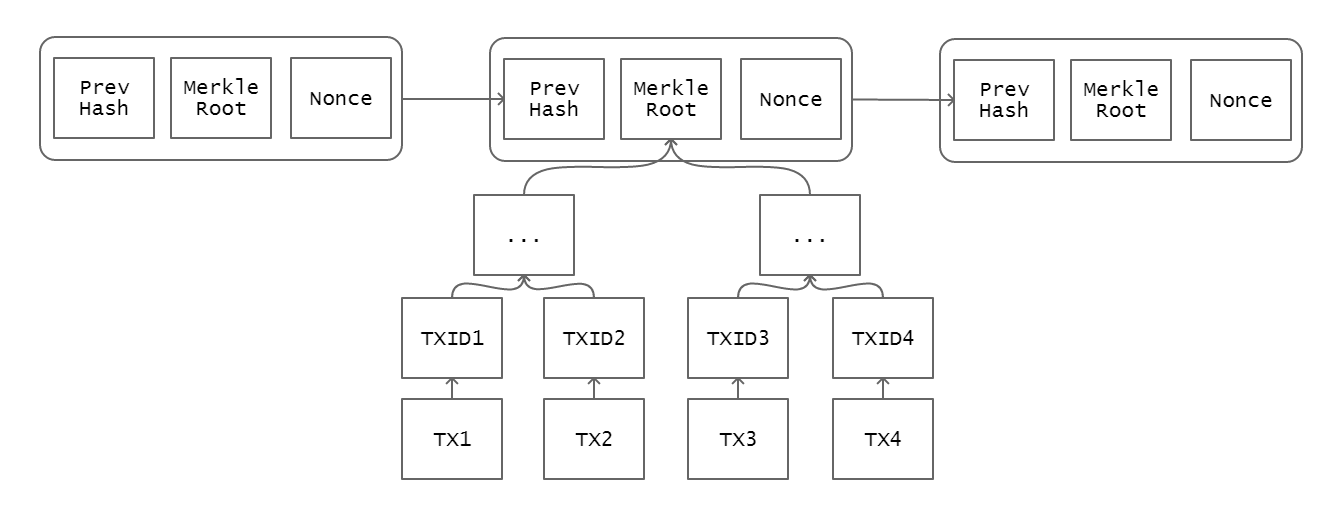
\includegraphics[width=\linewidth]{Images/bitcoin-chain-tx.png}
		\caption[Simplified scheme of the Bitcoin chain.]{Simplified scheme of the Bitcoin chain. The block header is richer and the transaction Merkle tree can be deeper}
		\label{fig:tx-chain}
	\end{center}
\end{figure}

The first block, called \textit{genesis block}, cannot include a previous timestamp, the field is set to $\{0\}^{256}$. The block include in the coinbase transaction the headline of The Times:
\begin{quotation}
"The Times 03/Jan/2009 Chancellor on brink of second bailout for banks"
\end{quotation}
It proves that the hash was computed after that newspaper was distributed. 
Since each block is a commitment of the previous block, every block is a commitment to the headline inserted by Nakamoto.

Every bitcoin owner \textit{without trusting other users} can broadcast \textit{without any permission} a transaction to the network, a miner include it in a new block which is appended to the chain or, in other words, it will be timestamped. Every network full node stores an entire copy of the chain to ensure the correctness of all bitcoin transactions ever made, thus the timestamp attestations are \textit{widely published}.  

Assuming the majority of the nodes does not collaborate to attack the network the cost of rewriting past blocks in the chain grows exponentially, making de facto impossible to change the chain. For this reason, provided not considering the very last blocks, the chain is said to be \textit{immutable}. 

Thus the Bitcoin network is a decentralized, trustless, permissionless notary. Its attestations are stored in a widely published and immutable timestamps chain, which defines the network (and vice versa). 

Bitcoin does something more than timestamping, Nakamoto consensus ensures that each UTXO is spent only once, thus to publish a transaction on the chain is necessary to follow the consensus rules. 
Anyway while playing in the consensus framework it's still possible to write arbitrary data inside a transaction.
As a premise note that a valid transaction can be mined, but not all valid transactions are relayed by nodes. To strengthen the network and the resilience of nodes only \textit{standard} transactions are relayed. This is a common practice between nodes, not a consensus rule, it may be changed if new useful transaction types are proposed. By the time of writing the standard transactions are:
\begin{itemize}
	\item Pay-to-Public-Key (P2PK)
	\item Pay-to-Public-Key-Hash (P2PKH)
	\item Pay-to-Script-Hash (P2SH)
	\item Multisig
	\item Null Data (OP\_RETURN)
\end{itemize}

In the following sections we show two ways to timestamp arbitrary data $d$ into the chain; the idea behind those is summarized in Figure \ref{fig:chain-data}.

\begin{figure}
	\begin{center}
		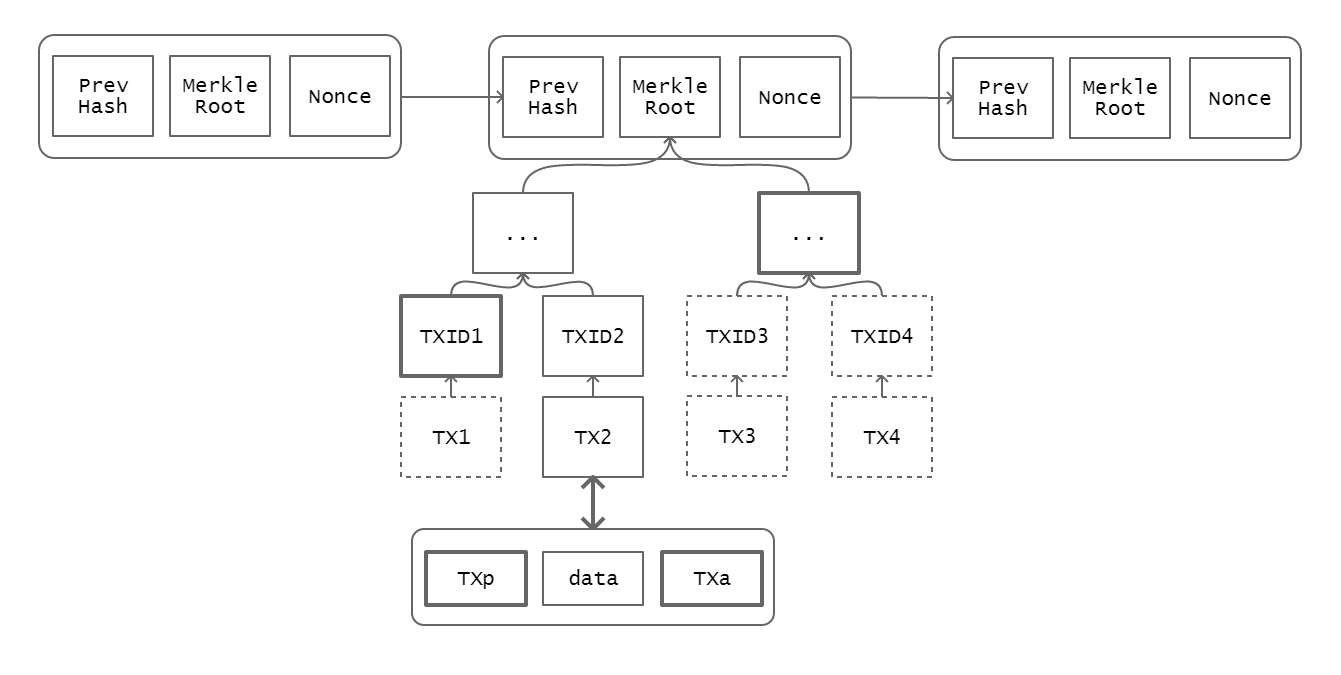
\includegraphics[width=\linewidth]{Images/bitcoin-chain-data-path.png}
		\caption[Commit arbitrary data in the Bitcoin chain.]{Commit arbitrary data in the Bitcoin chain. The transaction $TX_2$ includes some data, in the sense that $TX_2=TX_p||data||TX_a$.}
		\label{fig:chain-data}
	\end{center}
\end{figure}

\section{Address Commitment}
Consider the case of a transaction with one P2PKH output. In theory the output contains the hash value of the receiver public key computed applying SHA256 and then RIPEMD160, such value is called \textit{address}. The locking puzzle or \textit{pubkey script} is:
\begin{verbatim}
OP_DUP OP_HASH160 <PubKeyHash> OP_EQUALVERIFY OP_CHECKSIG
\end{verbatim}
The receiver, who knows the corresponding private key can redeem the bitcoin locked with an unlocking script or \textit{signature script} of this kind:
\begin{verbatim}
<sig> <pubkey>
\end{verbatim} 
To provide a timestamp for the data $d$ it is possible to compute the RIPEMD160 hash of $d$ and put it in place of the public key hash:
\begin{verbatim}
OP_DUP OP_HASH160 <DataHash> OP_EQUALVERIFY OP_CHECKSIG
\end{verbatim}
However this pubkey script is not redeemable (unless $d$ is a public key with known private key). Hence the bitcoin associated to this UTXO are lost, but a commitment to $d$ will be timestamped in the chain. 
This technique can also be used to prove that some bitcoin have been destroyed, called \textit{proof-of-burn}.

Even though is a viable and working solution this technique should be avoided, the burned output will stay forever in the database of the UTXO stored by every full node, called \textit{mempool}. If this happens consistently, it will bloat the mempool, adding an additional burden in running a full node, which is not good for the decentralization of the network.

% script op code
\section{OP\_RETURN}
To solve the UTXO bloat problem, with the Bitcoin Core 0.9.0 release, a new script opcode, OP\_RETURN. An OP\_RETURN change creates a \textit{provably-prunable} output, with script pubkey:
\begin{verbatim}
OP_RETURN <Data>
\end{verbatim}
Such output is provably unspendable, thus it will probably have zero bitcoin locked in, unless used for \textit{proof-of-burn}. The data field can be at most 80 bytes of arbitrary data. 

OP\_RETURN is used for different purposes, writing raw data on the chain, adding information related to assets linked to a coin or timestamping. Sometimes the data field starts with a prefix indicating if a second layer protocol is being used \cite{DBLP:conf/fc/BartolettiP17}. 

To create a timestamp for some data $d$ with arbitrary size one should add to his transaction an OP\_RETURN change followed by the hash value of $d$ with zero bitcoin associated. If the hash function used has a 32 bytes output, this increases the size of his transaction by 43 bytes (amount 8 bytes, length script pubkey 1 byte, OP\_RETURN 1 byte, length data field 1 byte, data 32 bytes) leading to a lower fee (measured in sat/byte\footnote{After segwit the correct metric to use is sat/vbyte instead of sat/byte}) which may slow down confirmation time or may lead the user to increase the overall fee, thus including an OP\_RETURN \textit{has a cost}.

In addition it is important to point out that when one wants to timestamp he has also to perform a bitcoin transaction. It may be a transaction that he would have done anyway, but in case these two needs does not coincide he has to send some bitcoins to himself adding the OP\_RETURN change to actually write something on the chain.
Moreover transactions including OP\_RETURN are easy to spot, hence malicious miners may decide to censor those. A solution is using address commitment, which can be censored only by censoring all the UTXO spendable by all the users who want to timestamp data, which is extremely hard.
Having said that, if there is no fear of censorship, presumably in most cases, OP\_RETURN is the correct tool for timestamping.

\chapter{State of the Art of Trustless Timestamping}
\label{chpr:state-of-art}
We analysed the reasons why Bitcoin chain is a valid tool to produce timestamps of arbitrary data and we showed two procedures to create such proofs.
However each one may follow his own set of rules to create and formalize proofs. 
One can use a different set of commitment operations and time attestations or the same set but formalized in a different way, or even a mixture ot the preceding cases. 
Although various set of rules may be valid and completely reasonable, such situation would be a nightmare for users, both creators and verifiers; during the creation procedure one may ask himself if challenger will retain his proof correctly formalized, verifiers should equip themselves with several tools increasing the cost of verifying proofs.
In addition this setting has huge security issues: an higher number of accepted formalizations increases the surface of attack through which proofs may be corrupted. 

Moreover Bitcoin chain is not the only place where to bind attestation in a trustless manner. 
There are other similar technologies that can be used as a notary with analogous techniques, for instance Litecoin, Ethereum or MimbleWimble.
Although timestamping with other chains is possible, it is fundamental to realize that it changes the security of the time attestations.
Each chain has its own rules and its own community behind, in some settings some assumptions may be weaker or false, while in others they may be an improvement.
For each specific case one should realize which is the best notary to use in order to properly address the problem.

For these reasons is important to have a common an shared standard to agree on the format used to create timestamps. 
Such standard should be open source to let everyone analyse its security and contribute to it with improvement proposals.

In 2012 Peter Todd started working on \textit{OpenTimestamps} \cite{OTSWeb, OpenTimestampsGithub, OTSannouncment}, a project that provides a solution to the above issues.

\begin{quotation}
	OpenTimestamps aims to be a standard format for blockchain timestamping. The format is flexible enough to be vendor and blockchain independent.
\end{quotation}

In the following years other developers contributed to the source code improving the standard with more libraries, features and implementations. 

\section{OpenTimestamps as a Standard}
OpenTimestamps defines a standard for creating a proof that can be verified in an easy way and that is not prone to inconsistent behaviours. The definition comes from the implementation, precisely from the python library which is currently taken as a reference by the other libraries.
Proofs consist in a sequence of commitment operations heading to at least one time attestation. 

Commitment operations take one (unary) or two (binary) inputs to produce a single output. Note that a binary operation can be turned in a unary operation by fixing one of the inputs. The available operations are:
\begin{itemize}
	\item
	\verb|OpAppend| binary
	\item \verb|OpPrepend| binary
	\item \verb|OpReverse| unary, may get removed\footnote{https://github.com/opentimestamps/python-opentimestamps/issues/5}
	\item \verb|OpHexlify| unary
	\item \verb|OpSHA256| unary, cryptographic
	\item \verb|OpRIPEMD160| unary, cryptographic
	\item \verb|OpSHA1| unary, cryptographic
	\item \verb|OpKECCAK256| unary, cryptographic
\end{itemize}

Time attestations are time-attesting signature, they link a commitment to an event which has a time associated to. As of writing, the available ones are:
\begin{itemize}
	\item \verb|UnknownAttestation| Placeholder for attestations that aren't support
	\item \verb|PendingAttestation| Commitment has been recorded in a remote server for future attestation
	\item \verb|BitcoinBlockHeaderAttestation| Signed by the Bitcoin blockchain: the commitment digest will be the merkleroot of the blockheader
	\item \verb|EthereumBlockHeaderAttestation| Signed by the Ethereum blockchain: the commitment digest will be the merkleroot of the blockheader\footnote{Ethereum attestations were developed for a PoC proving the flexibility of the protocol, however they are in the \textit{dubious} module of the OpenTimestamps repository, the reason given is:
		\begin{quotation}
			... Ethereum has changed repeatedly in the past due to consensus failures and forks; as of writing the Ethereum developers plan to radically change Ethereum's consensus model to proof-of-stake, whose security model is at best dubious.
	\end{quotation}}
	\item 
	\verb|LitecoinBlockHeaderAttestation| Signed by the Litecoin blockchain: the commitment digest will be the merkleroot of the blockheader
\end{itemize}
In the case of a single attestation, a proof is an ordered list of unary operations ending with a time attestation.  
However timestamps may have more than one attestation, in fact they are not limited to be linear lists of operations, instead they can be structured as a \textit{tree} with $d$ as the root, commitment operations as edges and attestations as leaves.
This enables the possibility to attach different attestations to a proof, with possibly completely different meanings.
A proof is conveniently serialized in a receipt, which is conventionally stored in a file whose name ends with \verb|.ots|;
let's examine an example of a receipt for a file \verb|test.txt| containing \verb|b'Hello World!\n'|. 
Its receipts \verb|test.txt.ots| is:
\begin{Verbatim}[frame=single]
File sha256: 03ba204e50d126e4674c005e04d82e84c21366780af1f43bd
             54a37816b6ab340
Timestamp:
ripemd160
prepend 0100000001e482f9d32ecc3ba657b69d898010857b54457a904979
        82ff56f97c4ec58e6f98010000006b483045022100b253add1d1cf
        90844338a475a04ff13fc9e7bd242b07762dea07f5608b2de36702
        2000b268ca9c3342b3769cdd062891317cdcef87aac310b6855e9d
        93898ebbe8ec0121020d8e4d107d2b339b0050efdd4b4a09245aa0
        56048f125396374ea6a2ab0709c6ffffffff026533e60500000000
        1976a9140bf057d40fbba6744862515f5b55a2310de5772f88aca0
        860100000000001976a914
append 88ac00000000
# Bitcoin transaction id
7e9f0f7d9daa2d9e51b2e22f4abe814c3f90539afa778a9bef88dc64627cb2
ec
sha256
sha256
prepend a987f716c533913c314c78e35d35884cac943fa42cac49d2b2c69f
        4003f85f88
sha256
sha256
prepend dec55b3487e1e3f722a49b55a7783215862785f4a3acb392846019
        f71dc64a9d
sha256
sha256
prepend b2ca18f485e080478e025dab3d464b416c0e1ecb6629c9aefce8c8
        214d042432
sha256
sha256
append 11b0e90661196ff4b0813c3eda141bab5e91604837bdf7a0c9df37d
       b0e3a1198
sha256
sha256
append c34bc1a4a1093ffd148c016b1e664742914e939efabe4d3d3565159
       14b26d9e2
sha256
sha256
append c3e6e7c38c69f6af24c2be34ebac48257ede61ec0a21b9535e44432
       77be30646
sha256
sha256
prepend 0798bf8606e00024e5d5d54bf0c960f629dfb9dad69157455b6f26
        52c0e8de81
sha256
sha256
append 3f9ada6d60baa244006bb0aad51448ad2fafb9d4b6487a0999cff26
       b91f0f536
sha256
sha256
prepend c703019e959a8dd3faef7489bb328ba485574758e7091f01464eb6
        5872c975c8
sha256
sha256
append cbfefff513ff84b915e3fed6f9d799676630f8364ea2a6c7557fad9
       4a5b5d788
sha256
sha256
prepend 0be23709859913babd4460bbddf8ed213e7c8773a4b1face30f8ac
        fdf093b705
sha256
sha256
verify BitcoinBlockHeaderAttestation(358391)
# Bitcoin block merkle root
8a1b66ecb7cbd07d8139a7e7d7f2c41aab1f5009b8364aaf61d03ad245e47e
00
\end{Verbatim}
The recepit is attesting that the file whose hash is \verb|03ba204e...| is committed into the block header number 358391, which has the \verb|nTime| field set to \verb|"May 28, 2015, 17:41:18 +0200"|. This means that the file existed prior to that time, still this is not completely safe: we are assuming that the miner has not lied \cite{TimeInaccuracy}. However he cannot put an extremely different date and he does not have a great incentive to put a false timestamp, nevertheless, we stay conservative and say that the data contained in the file existed prior to May 28, 2015.

This timestamp was created with an address commitment, to clarify how it is committed in the chain in Table \ref{tab:ots-ex} it is shown the receipt execution.
At the end, the value remaining on the stack is tested against the transaction Merkle root of block 358391. 
If they are equal the proof is correct.

\begin{table}
\begin{center}
\begin{tabular}{|p{3cm}|p{4cm}|}
	\hline
	\textbf{Operation} & \textbf{Object on the stack} \\ \hline
 & file \\ 
	\verb|sha256| & hash of the file \\ 
	\verb|ripemd160| & address commitment \\ 
	\verb|prepend 0100...| &  \\ 
	\verb|append 88ac...| & raw transaction \\ 
	\verb|sha256| &  \\ 
	\verb|sha256| & TXID in little endian \\ 
	\verb|...| &  \\ 
	\verb|sha256| &  \\ 
	\verb|sha256| & transactions merkle root \\ \hline
\end{tabular}
\end{center}
\caption[OpenTimestamp receipt execution.]{OpenTimestamp receipt execution.}
\label{tab:ots-ex}
\end{table}
The raw transaction of the example is:
\begin{Verbatim}[commandchars=+\[\], frame=single]
0100000001e482f9d32ecc3ba657b69d898010857b54457a90497982ff56f9
7c4ec58e6f98010000006b483045022100b253add1d1cf90844338a475a04f
f13fc9e7bd242b07762dea07f5608b2de367022000b268ca9c3342b3769cdd
062891317cdcef87aac310b6855e9d93898ebbe8ec0121020d8e4d107d2b33
9b0050efdd4b4a09245aa056048f125396374ea6a2ab0709c6ffffffff0265
33e605000000001976a9140bf057d40fbba6744862515f5b55a2310de5772f
88aca0860100000000001976a914+underline[1df8859e60bc679503d16dcb870e6ce91a]
+underline[57e9df]88ac00000000
\end{Verbatim}
It can be decoded with the Bitcoin Core client with:
\begin{verbatim}
$ bitcoin-cli decoderawtransction <raw-transaction>
\end{verbatim}
Decoding the transaction one can see the commitment address\footnote{It is possible to verify that it is still unspent.}:
\begin{verbatim}
13jUKAuPDfgVPVgsVbeKVNWBv6wAh31vkN
\end{verbatim}
which is the base58 encoding of:
\begin{verbatim}
1df8859e60bc679503d16dcb870e6ce91a57e9df
\end{verbatim}
which can be spotted inside the transaction.

Moving forward from the example it is possible to define procedures to include the timestamp in the Bitcoin chain, create and verify the corresponding proof as outlined in Algorithm \ref{alg:create-timestamp}.
\begin{algorithm}
\caption{Create timestamp on the Bitcoin chain}
\label{alg:create-timestamp}
\begin{algorithmic}[1]
\Procedure{IncludeTimestamp}{$d$}
\Comment{$d$ data to timestamp}
\State choose sequence of commitment operations $S_d^C=[C_i]_{i=1}^n$
\State apply $S_d^C$ to $d$, obtain $C$
\Comment{$d$ to $C$}
\State include $C$ in a transaction $TX$
\State broadcast the transaction to the network
\State wait until the transaction is confirmed
\State \textbf{return} $d$, $S_d^C$, $C$, $TX$
\EndProcedure
\Statex 
\Procedure{CreateTimestamp}{$d$, $S_d^C$, $C$, $TX$}
\State decompose the transaction, $TX = TX_p||C||TX_a$
\State $S_C^{TXID} = [\verb|prepend | TX_p,\verb| append | TX_a,\verb| sha256|,\verb| sha256|]$
\Statex
\Comment{$C$ to TXID}
\State find the block $B$ including $TX$
\State store $B$ transactions Merkle root $MR$ and height $H$
\State retrieve the Merkle path $S_{TXID}^{MR} \gets [C^{TXID}_i]_{i=1}^{n_{TXID}}$
\Comment{TXID to $MR$}
\State $proof \gets S_d^C + S_C^{TXID} + S_{TXID}^{MR}$ 
\Comment{join the commitment operations}
\State attach at the end of $proof$ \verb|BitcoinBlockHeaderAttestation(H)|
\State \textbf{return} $proof$
\EndProcedure
\Statex
\Procedure{VerifyTimestamp}{$d$, $proof$, $MR$}
\Statex
\Comment{$MR$ is retrieved from a \textit{trustworthy} source}
\State apply $proof$ to $d$, obtain $MR_V$
\Comment{execute commitment operations}
\If{$MR = MR_V$}{\textbf{ return }\verb|TRUE|}
\Comment{verify attestation}
\Else{\textbf{ return }\verb|FALSE|}
\EndIf
\EndProcedure
\end{algorithmic}
\end{algorithm}
The procedures could be easily generalized to more general settings, for instance to timestamp on another chain with slightly different rules.
It is important to highlight that the creator of the proof should always verify its correctness right after the creation. If the verification is successful he can store the file containing the proof in several insecure places, since it does not reveal anything more than the hash of the timestamped data, and store the file containing the data in a secure (if he needs) location; when challenged to prove the existence of that data prior to a certain time he will provide data and the corresponding timestamp to who he needs to convince.

\section{OpenTimestamps as a Scalability Solution}
As we have seen in the previous section, to create a timestamp is necessary to do a transaction. 
To timestamp multiple files it is possible to commit those in a single hash value using a Merkle tree. As a result, the initial part of each proof will have different operations, going through different branches of the tree, while, from the transaction on, the operations will be identical.

However, each time one has to timestamp, he has to do a bitcoin transaction, which is not sustainable if too many people have timestamp needs: it implies an effort for the network and higher fees for all the users.

The solution proposed by the OpenTimestamps developers includes a \textit{centralized trust-minimized} system to aggregate timestamps, it involves an \textit{aggregation server} and a \textit{public calendar server} which actually timestamp.
Their operation is descibed in Algorithm \ref{alg:calendar-working}.

\begin{algorithm}
	\caption{Client - aggregator - calendar simplified working}
	\label{alg:calendar-working}
	\begin{algorithmic}[1]
		\State clients send data to timestamp to the aggregator\Comment{timestamp requests}
		\State aggregator \Call{merklelize}{} requests received each second\Comment{aggregation}
		\State aggregator sends to calendar the Merkle tip to timestamp
		\State calendar promise he will timestamp the tip\Comment{pending attestation}
		\State aggregator sends back to clients incomplete proof until the tip
		\State calendar aggregates pending tips in a merkle tree\Comment{aggregation}
		\State calendar sends a transaction including a merkle tip\Comment{timestamp}
		\State the transaction gets confirmed\footnotemark \Comment{attestation complete}
		\State clients ask to the calendar to upgrade the timestamp\Comment{upgrade}
		\State calendar sends back clients the complete proofs
		\State clients verify their proofs\Comment{verification}
	\end{algorithmic}	
\end{algorithm}
\footnotetext{As pointed out in Section \ref{bitcoin}, a transaction is considered confirmed when it is 6 or more blocks deep.}

Clients do not send their data directly, instead they send salted hash values of the data, so the aggregator does not dig into their privacy.
At the first aggregation phase the aggregator append to each value received by clients a random nonce, so that a client sending malicious data instead of an hash do not pollute the proof of the leaf adjacent to his.
This system is trust-minimized beacause the clients trust that the calendar will create timestamp for them. Both calendar and aggregator can censor them, sending back incorrect proofs or malicious data. However once the calendar has sent them a correct proof they are fine, the proof will be valid forever regardless of any future bad behaviour of the aggregator or calendar.

The OpenTimestamp standard supports multiple branch for the commitment operations to include multiple attestations inside a single proof. With this feature one request can be forwarded to multiple public calendars, giving the redundancy that mitigates the problem when a calendar server is down and lowering the trust put in each single calendar.

\begin{figure}
	\begin{center}
		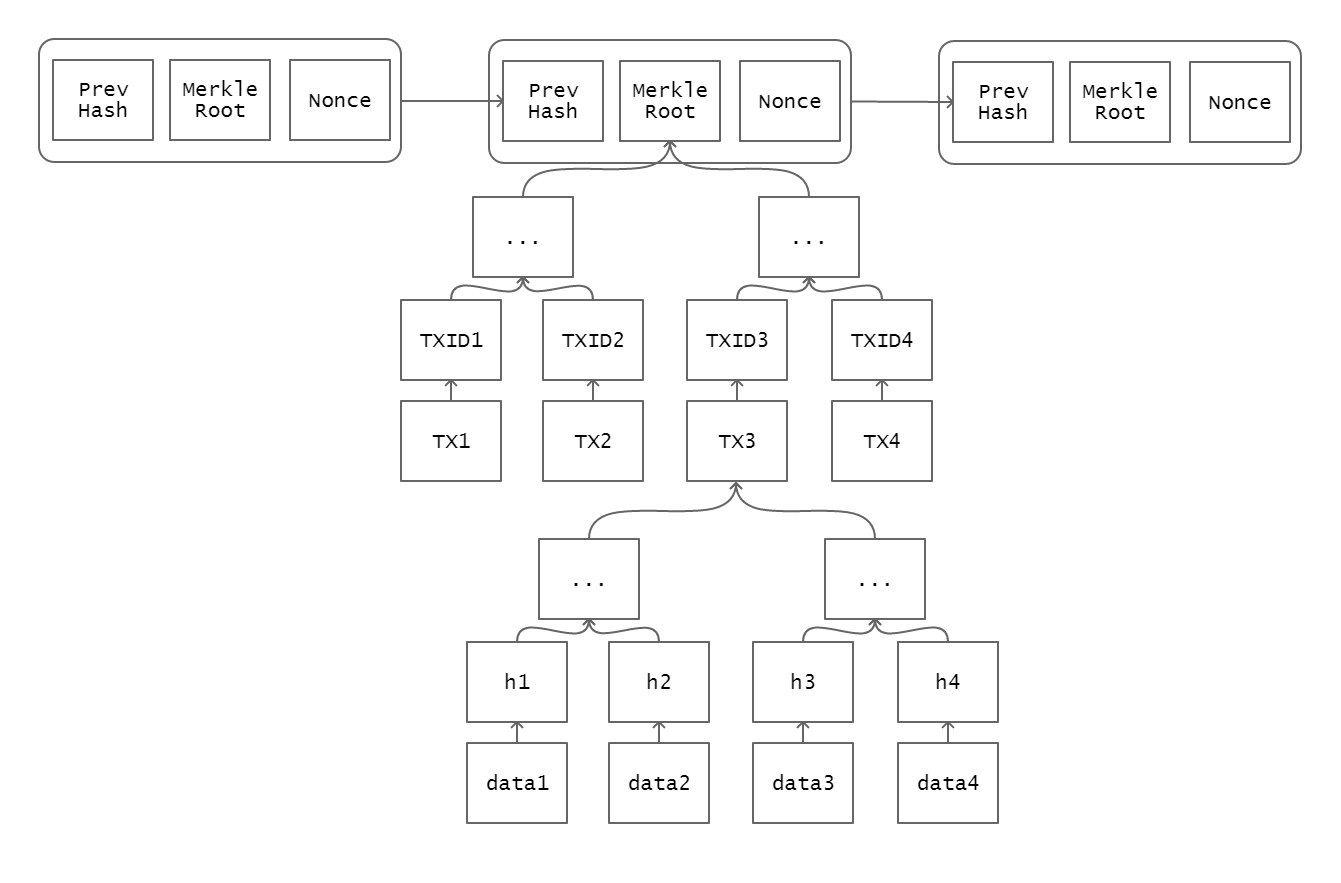
\includegraphics[width=\linewidth]{Images/bitcoin-chain-calendar.png}
		\caption[Calendar timestamping.]{Calendar timestamping. $TX_3$ is the transaction made by the calendar, it includes a commitment to $\{data_i\}_{i=1}^n$ obtained with a Merkle tree. Note that transaction must follow the consensus rules to be included in the chain, instead data are completely arbitrary.}
		\label{fig:chain-calendar}
	\end{center}
\end{figure}

A calendar spends its own bitcoin to do a transaction, this implies that he won't be able to perform an extremely high number of transactions, leading to less frequent timestamps. As of writing, the calendars use the \textit{replace by fee} (\textit{RBF}) mechanism to spend a fix amount of bitcoin each day. In Algorithm \ref{alg:calendar-rbf} is described a simplified scheme of its working.
This procedure makes the calendar expenditures fixed: each day has approximately 144 block, so the amount spent in fee per day is $144 \cdot a$, where $a$ is a fixed value set by who run the calendar.

Thus if the mean fee to get into the next block is high, then the calendar may wait several blocks before timestamping and clients will have to wait for a long time to have their receipt upgraded and their data timestamped. This issue can be addressed if someone is timestamping in place of the calendar, which could be facilitated by the technique we are showing in Chapter \ref{chpr:ec-commitments}. 

Despite all these considerations, the existence of public calendars is an extremely remarkable achievement for users: they enable clients to timestamp completely for free their own data. 
The solution involves some trust\footnote{Actually a client may implement a trustless system involving the calendar to timestamp his data. He would first ask the calendar to timestamp and then wait for the completed proofs; after a reasonable amount of time, if the calendar delivered what promised, then the client is fine, otherwise he timestamps by himself.}, but for a limited interval of time and with minimal possible downsides; once the proof is completed, it is not important if it was created through a central hub, it has the exact same respectability of any other proof. 
Furthermore the calendar learned nothing about the data timestamped since it received only an hash value. 
Ultimately the efficient aggregation reduces the burden caused to the network, making timestamping sustainable even on large scale.

\begin{algorithm}
	\caption{Calendar replace by fee}
	\label{alg:calendar-rbf}
	\begin{algorithmic}[1]
		\Procedure{calendarRBF}{$a,LT$}\Comment{step $a$, last timestamp $LT$}
		\State $fee \gets 0$
		\Repeat 
		\State $fee \gets fee + a$
		\State $S \gets \{h_i\}_{i=1}^n$ \Comment{collect clients timestamp requests}
		\State $MR \gets$ \Call{merklelize}{$S$}
		\State $TX \gets$ \Call{maketx}{$fee, MR$} \Comment{create transaction including $MR$}
		\State broacast $TX$
		\Until{$TX$ is mined}
		\State \textbf{return} $LT$ \Comment{$LT$ to restart the procedure}
		\EndProcedure
	\end{algorithmic}
\end{algorithm}

\chapter{Elliptic Curve Commitments}
\label{chpr:ec-commitments}
Elliptic curve cryptography is used in Bitcoin and in similar systems to secure the transactions. 
We will give a brief overview of this cryptosystem, then we show how an elliptic curve point can be a commitment, finally we describe the consequent practical timestamping applications with Bitcoin.  

\section{Elliptic Curve Public Key Cryptosystem}
We start with a general definition taken from \cite{Koblitz1987}\footnote{See Appendix \ref{app:A} for a more basic approach.},
\begin{mydef}
	An elliptic curve $E_K$ defined over a field $K$ of characteristic $\neq 2, 3$ is the set of solutions $(x,y)\in K^2$ to the equation
	\begin{equation}
	\label{ec-eq}
	y^2 = x^3 + ax + b, \quad a,b \in K
	\end{equation}
	together with a \textquotedblleft point at infinity\textquotedblright $\mathcal{O}$.
\end{mydef}
$\mathcal{O}$ is the projective closure of (\ref{ec-eq}) and may not be described in terms of two coordinates in $K$.
The points on $E_K$ form a group with identity element the point at infinity. The negative point $P \in E_K$ is the second point on $E_K$ having the same $x$-coordinate as $P$. Let $P_1=(x_1,y_1)$ and $P_2=(x_2,y_2)$ be two points on the curve, their sum $P_3=(x_3,y_3) = P_1 + P_2$ is given by:
\begin{equation}
x_3 = -x_1 -x_2 + \alpha^2, \quad 
y_3 = -y_1 + \alpha(x_1 - x_3),
\end{equation}
where
\begin{equation}
\alpha = \begin{cases}
			(y_2 - y_1)/(x_2 - x_1) & \textrm{if } P_1 \neq P_2, \\
			(3x_1^2 + a)/(2y_1) & \textrm{if } P_1 = P_2.
\end{cases}
\end{equation}
This \textit{addition} operation for elliptic curve points has a geometric interpretation for $K = \mathbb{R}$, from which the above more general algebraic formulae can be derived.

Using these formulae, one can compute a multiple $mP$ of a given point $P$ in polynomial time by means of $O(\log m)$ doubling and additions, e.g. $11P = P + 2(P + 2(2P))$. This operation is called \textit{scalar multiplication}.

In cryptography most applications use finite fields, in particular a finite field contains $p^m$ elements with $p$ prime and $m \geq 1$. We will confine ourselves to the case $m=1$. So let $K=GF(p)=\mathbb{F}_p =\mathbb{Z}_p  = \{0, 1, ..., p-1\}$, $K$ is a finite field, the points of $E_K$, together with the addition operation defined above, form a finite Abelian group. The elliptic curve becomes:
%cyclic or product of two cyclic groups
\begin{equation}
E_{\mathbb{F}_p}=\{(x,y)\in \mathbb{F}_p^2 \quad \textmd{s.t. }
y^2 = x^3 + ax + b \mod p, \quad a,b \in \mathbb{F}_p \} \cup \mathcal{O}
\end{equation}
Let $G \in E_{\mathbb{F}_p}$ be a conventional element of order $n$, called $generator$. The subgroup generated by $G$ is:
\begin{equation}
	\langle G \rangle = \{xG|x \in \mathbb{Z}_n\} \subseteq E_{\mathbb{F}_p}
\end{equation}
Which is a cyclic group isomorphic to $\mathbb{Z}_n$; in particular, if $n$ is prime, then $\langle G \rangle = E_{\mathbb{F}_p}$.

Computing the isomorphism from $\mathbb{Z}_n$ to $\langle G \rangle$ is efficient, it takes $O(\log n)$ group operations; while the opposite isomorphism is much harder to compute, at moment, the best algorithm known takes approximately $\sqrt{n}$ operations. The latter procedure is called discrete logarithm and it stands at the base of the cryptosystem, more precisely:
\begin{mydef}
	Elliptic Curve Discrete Logarithm Problem (ECDLP). Given an elliptic curve $E$ defined over $GF(q)$ and two points $P, Q \in E$, find an integer $x$ such that $Q = xP$ if such $x$ exists.
\end{mydef}
Elliptic curve cryptography is based on the premise that ECDLP is hard, actually it appears to be more intractable than DLP in finite fields.
The ECDLP difficulty enables a Diffie-Hellmann key exchange which precedes the ElGamal signature scheme, these techniques are at the foundations of the public key cryptosystem.
Fixed a point $P \in E_{\mathbb{F}_p}$, a \textit{public key} is a point $Q \in E_{\mathbb{F}_p}$ while its discrete logarithm $x$ w.r.t. $P$ ($xP=Q$) is the \textit{private key}.
Given $x$ is easy and fast to compute $Q$, while given $Q$ is infeasible to find $x$.

To classify different curves the Standard for Efficient Cryptography (SEC) proposed a set of parameter for elliptic curves over $\mathbb{F}_p$:
\begin{equation}
(p, a, b, G, n, h)
\end{equation}
\begin{itemize}
	\item $p$ prime defines the finite field $\mathbb{F}_p$
	\item $a, b \in \mathbb{F}_p$ define the curve $E_{\mathbb{F}_p}$
	\item $G\in E_{\mathbb{F}_p}\backslash \{\mathcal{O}\}$ is a generator of the group
	\item $n = |\langle G \rangle|$ is the order of the group (smallest $n>0$ s.t. $nG = \mathcal{O}$)
	\item $h = |E_{\mathbb{F}_p}| / n$ is the cofactor
\end{itemize}
Note that if $n$ prime, then $\langle G \rangle = E_{\mathbb{F}_p}$, thus $n = |E_{\mathbb{F}_p}|$, $h=1$.
Bitcoin uses the curve named $secp256k1$ with parameters
\begin{verbatim}
p = 0x FFFFFFFF FFFFFFFF FFFFFFFF FFFFFFFF FFFFFFFF FFFFFFFF 
       FFFFFFFE FFFFFC2F
a = 0
b = 7
G = (0x 79BE667E F9DCBBAC 55A06295 CE870B07 029BFCDB 2DCE28D9 
        59F2815B 16F81798, 
     0x 483ADA77 26A3C465 5DA4FBFC 0E1108A8 FD17B448 A6855419 
        9C47D08F FB10D4B8)
n = 0x FFFFFFFF FFFFFFFF FFFFFFFF FFFFFFFE BAAEDCE6 AF48A03B 
       BFD25E8C D0364141
h = 1
\end{verbatim}
With this curve some calculation becomes more efficient, like computing the modular square root ($\sqrt{x}=x^{\lfloor\frac{p+1}{4}\rfloor}\textmd{ mod }p$, since $p= 3 \textmd{ mod }4$) and the modular inverse ($x^{-1}=x^{p-2}\textmd{ mod }p$, since $p$ prime).

Looking at the generator above one may think that to store an elliptic curve point is necessary to use 32 bytes for the $x$-coordinate and 32 bytes for the $y$-coordinate. 
However it is not necessary to use all that space, infact it is possible to take advantage of the elliptic curve equation. Suppose $x \in \mathbb{F}_p$ is the $x$-coordinate of a point, then $y$ is given by $y^2 = x^3 + ax + b \quad \text{mod }p$, which, for $p$ prime, has exactly two solutions in $\mathbb{F}_p$, $y$ and $p-y$, one is odd and the other is even.
The solutions are easily computable thanks to the above formula.
Having consider this, to store an elliptic curve point $P$ one can store $P_x$ and the parity of $P_y$. 
In Bitcoin the compressed encoding of a point $P$ is given by a byte for the parity of $P_y$ ($02$ if even, $03$ if odd) followed by the bytes representing $P_x$, for instance the generator $G$ is encoded as follows:
\begin{verbatim}
G = 02 79BE667E F9DCBBAC 55A06295 CE870B07 029BFCDB 2DCE28D9 
       59F2815B 16F81798
\end{verbatim}

\section{A New Commitment Operation}

Combining conveniently elliptic curve points and hash functions, it is possible to create new commitment operations.
A similar technique was used for the first time for deriving public keys in deterministic wallets \cite{Max11},
then the concept of embedding a value in an elliptic curve point was exploited \cite{journals/corr/abs-1212-3257, Sidechain},
later it was reformulated in a more refined way \cite{PoePR, PoeIs}
suitable for the integration in OpenTimestamps.
Let's analyse how this new commitment operations are structured.

\begin{myprop}
	Let $E_{\mathbb{F}_p}$ be an elliptic curve defined on the finite field $\mathbb{F}_p$ with $p$ prime, $G \in E_{F_p}$ be the generator of the curve with order $n$ large prime. Let $h$ be a second-preimage resistant hash function, its input are somehow serialized in bits, its output are in $\{0,1\}^k$ and are interpreted as integers.
	Let $C$ be defined as follows:
	\begin{equation}
	\begin{split}
	C : \{0,1\}^* \times E_{\mathbb{F}_p}  & \rightarrow E_{\mathbb{F}_p} \\
	    m, P & \mapsto h(P||m)G + P
	\end{split}
	\end{equation}
	If $n$ is close to $2^k$, then $C$ is a commitment operation.
\end{myprop}
\begin{proof}
	First we show a direct proof that works when $P$ (or $P'$) is fixed then we show the general proof.
	\\
	Let $m,P$ and $C(m,P)$ be fixed.
	%Let $C(m,P)$ be a commitment to $m, P$.
	$\forall P' \in E_{\mathbb{F}_p}$ the problem is to find $m' \in \{0,1\}^*$ s.t. $C(m,P)=C(m',P')$ and $(m', P') \neq (m, P)$. 
	We want to show that such problem is infeasible.
	$m'$ satisfies $h(m'||P')G + P'=C(m,P)$.
	%The substitute value $m'$ needs to satisfy $h(m'||P')G + P'=C(m,P)$.
	Let $x$ be such that $xG = C(m,P) - P'$, with $0\leq x<n$. 
	%so $x=h(P'||m')\textmd{ mod }n$. The problem to find a second preimage $m'$ of $x$.
	Let $h_{P'}$ be defined as follows:
	\begin{equation*}
	\begin{split}
	h_{P'}:\{0,1\}^* & \rightarrow \{0,1\}^k\\
	m' & \mapsto h(m'||P')
	\end{split}
	\end{equation*}
	Consider the elements in $\{0,1\}^{k}$ equivalent to $x$ modulo $n$, namely $I_x=\{h \in \{0,1\}^k \approx \mathbb{Z}_{2^k} | h=x\textmd{ mod }n\}$.
	%Let $I_x=\{h \in \{0,1\}^k \approx \mathbb{Z}_{2^k} | h=x\textmd{ mod }n\}$ be the set of images of $h_{P'}$ suitable to find a second-preimage.
	Note that:
	\begin{equation*}
		|I_x|=\begin{cases}
				\lceil\frac{2^k}{n}\rceil & \textmd{if } x\geq n \\
				\lfloor\frac{2^k}{n}\rfloor & \textmd{if } x< n
		      \end{cases}
	\end{equation*}
	The problem is finding $h_{p'}(m')\in I_x$.
	Note that $h_{p'}$ is second-preimage resistant, since it is the composition of two functions with that property, $prepend(P')$ and $h$.
	Finally, if $n \approx 2^k$, the elements in $I_x$ are few (eventually a single one), thus finding $m'$ is infeasible because $h_{P'}$ is second-preimage resistant.
	%$I_x$ contains  $\lceil\frac{2^k}{n}\rceil$ or $\lfloor\frac{2^k}{n}\rfloor$ elements.
	%Hence to find a second-preimage one needs to find $m'$ s.t. $h_{P'}(m') \in I_x$. Note that $h_{P'}$ is second-preimage resistant, since it is the composition of two function with that property, $prepend(P')$ and $h$. Finally, if $n \approx 2^k$, the elements in $I_x$ are few (eventually a single one), thus finding $m'$ is unfeasible because $h_{P'}$ is second-preimage resistant.
	\\
	Now consider the case in which $P$ is not fixed.
	We model the hash function $h$ as a random oracle $H$ with range $\{0,1\}^k\approx \mathbb{Z}_{2^k}$.
	$H$ initially has an empty table. 
	When someone queries the oracle for a value $x \in \{0,1\}^*$,
	the oracle samples uniformly a random value $H(x)$ in $\mathbb{Z}_{2^k}$ and associate it with $x$.
	The oracle outputs $H(x)$ and annotate it on his table.
	If someone calls again the oracle for $x$ he will answer with $H(x)$.
	The oracle is queried by different entities for possibly different values.
	Queries for new values result in a new line in the table.
	Thus before querying $H$ for $x \in \{0,1\}^*$, we expect $H$ to output a uniform random value in $\mathbb{Z}_{2^k}$.
	\\
	Now suppose the  discrete logarithm is broken, so anyone can run the map $x \mapsto xG$ both ways.
	The map:
	\begin{equation*}
	\begin{split}
	\tilde{C} : \{0,1\}^* \times E_{\mathbb{F}_p}  & \rightarrow E_{\mathbb{F}_p} \\
	m, P & \mapsto H(P||m)G + P
	\end{split}
	\end{equation*}
	where $h$ is substituted by $H$. 
	If $P=xG$, it becomes:
	\begin{equation*}
	\begin{split}
	\hat{C} : \{0,1\}^* \times \mathbb{Z}_n  & \rightarrow \mathbb{Z}_n \\
	m, x & \mapsto (H(xG||m) + x)\textmd{ mod }n
	\end{split}
	\end{equation*}
	We show that $\hat{C}$ can be used as a random oracle.
	$H$ is uniformly random and independent from its inputs, 
	moreover the offset $x$ cannot affect that.
	Applying $\textmd{mod }n$ shrinks the range to $\mathbb{Z}_n$,
	still $\hat{C}$ can be used as a random oracle.
	Finally the output of $\hat{C}$, which is equivalent to $C$, is indistinguishable from the output of a random uniform distribution in $\mathbb{Z}_n$.
	Since $n$ is close to $2^k$ finding a second-preimage to $C(m,P)$ is infeasible. 
	%Now consider the case in which $P$ is not fixed.
	%Suppose we are able to find $x$ s.t. $P=xG$, the map $C$ can be seen as $m,x \mapsto x + h(xG||m)$ which is basically $m,x \mapsto x + \tilde{h}(x,m)$ for an opportune $\tilde{h}$.
	%If such map is a random oracle then we are done, since random oracles are second preimage resistant.
	%We assume $h$ is a random oracle, then also $\tilde{h}$ has the same feature, since it is independent from its input, moreover the offset $x$ does not affect the property. 
	%Hence we conclude that the map is a random oracle which gives second preimage resistance.
\end{proof}

The order $n$ has to be large so that $E_{\mathbb{F}_p}$ is rich enough to make the ECDLP intractable and to avoid shrinking the hash function codomain. Fixed $n$ the choice of $k$ should be made properly: if it is too low $h$ by itself will be too weak, if it is too high, $|I_x|$ will increase, weakening $C$. Hence a good compromise is choosing $n$ the closest possible to $2^k$.

The security of the commitment is given by the security of the hash function, and does not rely on the intractability of the ECDLP. Being able to compute the private key from the commitment is not enough to compute a second input committing to the same point, to do so it is necessary to able to find a second-preimage to an hash value.

With this commitment an elliptic curve point used for one purpose can be tweaked with $h(P||m)$ and, while still serving for the previous purpose, it can be a commitment to a value $m$. In fact suppose $x$ is the private key of $P$, $P=xG$, then $C(m,P)=(h(P||m)+x)G$. So the new private key is $(h(P||m)+x) \textmd{mod } n$ and, since $x$ is secret and $h(P||m)$ is a constant value, the resulting key is still secret.
So each time an elliptic curve point is written, we can encapsulate it in a commitment to an arbitrary value.
This technique may be extended to more general cases, but we will treat only the case of elliptic curves.

Several hash functions and elliptic curves can be used, considering we want to use Bitcoin as notary, we will focus an a particular case with $h=$ SHA256 and $E_{\mathbb{F}_p}=secp256k1$ since Bitcoin itself relies on the assumption that this hash function and this elliptic curve are not broken.
Moreover, the order of the curve $n$ is extremely close\footnote{Assuming that a generic output $x$ of SHA256 is indistinguishable from a sampling from an uniform distribution in $\mathbb{Z}_{2^{256}}$, then $\mathbb{P}(x\geq n)=1-\frac{n}{2^{256}}\approx 10^{-33}$. So the chance to choose $(P||m)$ leading to $|I_x|=2$ is almost zero.} 
to the cardinality of the hash function codomain $2^{256}$. This commitment operation is called \verb|OpSecp256k1Commitment|.

Furthermore, to use this operation in as OpenTimestamp receipt, it has to be an unary operation, hence it will take as input $P||m$ and will return the $x$-coordinate of $C(m P)$ as output, both in bytes. More precisely it will operate as described in Algorithm \ref{alg:opsecp256k1}.
\begin{algorithm}
	\caption{Commitment to a $secp256k1$ point using SHA256}
	\label{alg:opsecp256k1}
	\begin{algorithmic}[1]
	\Procedure{OpSecp256k1Commitment}{$c$}\Comment{$c$ is $P||m$}
	\State $P,m \gets$ \Call{decode}{$c$}\Comment{for bad $c$  return error}
	\State $tweak \gets h(P||m)$\Comment{interpreted as an int}
	\State $Q \gets tweak G + P$
	\State \textbf{return} \Call{encode}{$Q_x$}\Comment{output in bytes}
	\EndProcedure
	\end{algorithmic}
\end{algorithm}
It can be used for several purposes, however, for this work, we focus only on timestamping.

\section{Timestamping Applications}
On the Bitcoin chain, elliptic curve points are used as public keys locking bitcoins or as part of the signature. The first case lead to the \textit{pay-to-contract} technique, the second to \textit{sign-to-contract}. We will analyse both uses and we will explain which one should be preferred.

These names owe their origin to the first application for which they were though: associate a \textit{contract} to an elliptic curve point. 
The term contract may seem misleading, but it turns out to be useful dealing with \textit{sign-to-contract}, since it let us distinguish between the message signed and the contract committed.

\subsection{\textit{pay-to-contract}}
Public keys are elliptic curve points, here we show how they could commit to a value while still maintaining the secrecy of the private key.

We illustrate it through an example. 
Alice needs to send Bob some bitcoins. 
Bob has public key $P=xG$. 
Bob wants to timestamp the message $m$. 
Bob computes $Q=h(P||m)G+P$. 
Bob tells Alice that his public key is $Q$.
Alice broadcasts a transaction sending bitcoins to $Q$, for instance she uses a P2PK publishing on the chain:
\begin{verbatim}
script pubkey:
<Q> OP_CHECKSIG
\end{verbatim}
Bob can spend the bitcoin locked in this script because he knows $P$, $m$ and $x$, so he can compute the private key corresponding to $Q$, that is $(h(P||m)+x) \textmd{ mod } n$.
To create the timestamp proof he has to decompose the transaction including $Q$ and create a proof that will look like:
\begin{verbatim}
prepend P
secp256k1commitment
prepend TX_p
append TX_a
sha256
...
sha256
verify BitcoinBlockHeaderAttestation(block)
\end{verbatim} 
In the case of P2PKH, the committed public key is hashed as shown in the following real example, where \verb|b'Pay to contract!\n'| is timestamped: 
\begin{Verbatim}[frame=single]
File sha256: 47257ff8c07f55a2e697ab9d89e47b471f60ab3f6883ed05
             44561b2a39a26140
Timestamp:
prepend 02a1e5aafa5082d035c659143660b2526a4ba60d4ab5b2e603905
        0eae9444d56ee
secp256k1commitment
prepend 02
sha256
ripemd160
prepend 01000000018fccf63afda6cf748acfe946a344f417bd4a8994bc1
        bf933501a87986363464c000000006a47304402207724a6a96e91
        a10821ee0c6db30a2f764ba8bd1dcdc82812fb958f6b91e97a4a0
        22062db4df7205e6c97d9833f7ab0d597b7685e8320bb2031f57a
        a6981cd2f626a40121030eb7a6c01ab07d3bfe598c295e9edfbeb
        38e5d2df7320f16b4349fb89a975ab7fdffffff02e22000000000
        00001976a914d8da7633fe644eb12617b2b1f0ba3f0461a2bc5e8
        8ac10270000000000001976a914
append 88ac4ed90700
# Bitcoin transaction id
1b07d87e0f4e32d545932bf03e306d1532bc7d91f56e81dee81b7cd0b707a9
9d
sha256
sha256
prepend 9d12daa914a3d39cd25b36516383683aae3ac6f873b952bbab11cc
        417650bb49
sha256
sha256
prepend 0123f36690131b2416d32a7e6c3c63110d9d77873911f71ad22740
        b398a13874
sha256
sha256
append 9f45bbc92ac4ef65b5e5bfad479da46c400f6e7ab96217a20b4e08d
       bfab47a45
sha256
sha256
prepend 949c83f6b502ec75c4647da6ed4e26d181de07b325eac75881de7b
        b715a44c50
sha256
sha256
prepend 2ef8ff1aad05e891215698fe237546c73347967419f33d08baf0d9
        71ab00004d
sha256
sha256
append 9bf69359a440f6a15a2a11adb1f257c96089ad27ef66e57a19056e3
       3ecc1795b
sha256
sha256
prepend c1c9bb36792745df3967704dd5d15899bab47b0a9de35486eb339a
        b4d00ff340
sha256
sha256
append c0b13e8aa4dc85a8256efb03272dea659e41fc67bc2f44add154111
       c68f700be
sha256
sha256
append 1bf843d12afce2a7b02ebe1f083eb2c39a101a63474a622724f609a
       3f08f8c7f
sha256
sha256
append a29eece3554c358e5df3901478c8670c71dbafe4e435cf660a18bb6
       09d6d025d
sha256
sha256
append aa2c4696c3b75f73713345a7e4279805a9519fd067835769b41dcf7
       88d6a7c96
sha256
sha256
prepend f7290a75923a0c54e87a50bbeff75f614437ed799347a46053a633
        8dba42b5c7
sha256
sha256
verify BitcoinBlockHeaderAttestation(514394)
# Bitcoin block merkle root
be6859c5093de84a06e495b6621054616ce5bf7a38f24374a225d0da0c0de8
88
\end{Verbatim} 
The raw transaction with the above TXID is 
\begin{Verbatim}[commandchars=+\[\], frame=single]
01000000018fccf63afda6cf748acfe946a344f417bd4a8994bc1bf933501a
87986363464c000000006a47304402207724a6a96e91a10821ee0c6db30a2f
764ba8bd1dcdc82812fb958f6b91e97a4a022062db4df7205e6c97d9833f7a
b0d597b7685e8320bb2031f57aa6981cd2f626a40121030eb7a6c01ab07d3b
fe598c295e9edfbeb38e5d2df7320f16b4349fb89a975ab7fdffffff02e220
0000000000001976a914d8da7633fe644eb12617b2b1f0ba3f0461a2bc5e88
ac10270000000000001976a914+underline[57529515dc2e14701374eb65f0191b61ecfd]
+underline[d0e3]88ac4ed90700
\end{Verbatim}
Where the commitment to the data is underlined.

This technique is completely viable, but it has a relevant issue.
Almost all bitcoin wallets (software to manage private keys) use a deterministic derivation for creating new keys \cite{BIP32}. An initial value is generated at random using a cryptographically secure procedure, this value is called \textit{seed} and sometimes encoded as a list of words from a given dictionary. The keys are obtained from the seed using the specifications given by BIP32 and they are something like $h(seed||number)$. This procedure make possible to completely recover a wallet from the seed only, so if a user wants to use his wallet from another device he just need to remember the seed and all his private keys will be reconstructed.
Using pay-to-contract actually Bob goes outside of the BIP32 derivation. So if he looses $m$ or $P$ he won't be able to spend the bitcoin locked by $Q$. For this reason the use of \textit{pay-to-contract} for mere timestamping purposes should be limited.

In the case of a P2PKH, a timestamp made with \textit{pay-to-contract} reveals the public key which is the preimage of the receiving address. 
The public key will be revealed anyway when the corresponding output will be spent, but, if it is still unspent, such disclosure may be an undesired feature. 
In addition, when spending that UTXO, the public key is actually written in the chain, giving another anchoring point to create a different timestamp; this timestamp is just another path from the data to the chain, but it is not really useful since it cannot precede the other timestamp.

\subsection{\textit{sign-to-contract}}
The other place where elliptic curve points are published in the chain is the signature. Bitcoin uses the elliptic curve digital signature algorithm, ECDSA\footnote{\textit{sign-to-contract} works also with other signature schemes involving elliptic curves, like Schnorr signature.}, that works as detailed in Algorithm \ref{alg:ecdsa-sign}.
\begin{algorithm}
	\caption{ECDSA signature}
	\label{alg:ecdsa-sign}
	\begin{algorithmic}[1]
		\Procedure{ECDSAsig}{$x, m$}\Comment{$x$ private key signing}
		\Statex \Comment{$m$ 32 bytes message to be signed}
		\State $k \in_R \mathbb{Z}_n \backslash \{0\}$ \Comment{select $k$ at random in $\{1,..., n-1\}$}
		\State $R \gets k G$
		\State $r \gets R_x \textmd{ mod }n$\Comment{if $r=0$, fail}
		\State $s \gets k^{-1}(m + rx) \textmd{ mod }n$\Comment{if $s=0$, fail}
		\State \textbf{return} $(r,s)$
		\EndProcedure
	\end{algorithmic}
\end{algorithm}
The value $k$ is called nonce or \textit{ephemeral private key}, $R$ is called \textit{ephemeral public key}.

A signature is a couple of integers in $\{1,...,n-1\}$, the first one is the $x$-coordinate (mod $n$) of the ephemeral public key.
The idea of \textit{sign-to-contract}, exploited in Algorithm \ref{alg:ecdsa-s2c}, is to tweak $R$, so that the first part of the signature will be a commitment to (also) another message, the contract $c$.
\begin{algorithm}
	\caption{ECDSA \textit{sign-to-contract} (s2c)}
	\label{alg:ecdsa-s2c}
	\begin{algorithmic}[1]
		\Procedure{ECDSAs2c}{$x, m, c$}\Comment{$x$ private key signing}
		\Statex \Comment{$m$ 32 bytes message to be signed}
		\Statex \Comment{$c$ contract to commit}
		\State $k \in_R \mathbb{Z}_n \backslash \{0\}$ \Comment{select $k$ at random in $\{1,..., n-1\}$}
		\State $R \gets k G$
		\State $tweak \gets h(R||c)$\Comment{interpreted as an int}
		\State $e \gets (k + tweak) \textmd{ mod }n$ \Comment{if $e=0$, fail}
		\State $Q \gets tweak G + R$
		\State $q \gets Q_x \textmd{ mod }n$\Comment{if $q=0$, fail}
		\Statex \Comment{if $q \neq Q_x$, commitment fail}
		\State $s \gets e^{-1}(m + qx) \textmd{ mod }n$\Comment{if $s=0$, fail}
		\State \textbf{return} $(q,s), R$\Comment{$R$ is needed to prove the commitment}
		\EndProcedure
	\end{algorithmic}
\end{algorithm}

Let's examine a real timestamp for the data \verb|b'Sign to contract\n'| made with the described technique.
\begin{Verbatim}[frame=single]
File sha256: dd60bcfecd023823efdcb8d8a5b04939111ef82dc1d674320
             7e164e5aab08844
Timestamp:
append eb7e45e783d98504b2e64342b0bea3f5
sha256
prepend 0372a1fb359a24eab552e8c588f84b7e08144bbb10e87bfa6db649
        8c7df730e867
secp256k1commitment
prepend 01000000018fccf63afda6cf748acfe946a344f417bd4a8994bc1b
        f933501a87986363464c010000006a4730440220
append 022057db028ba602b467d09f67b6a6327d3219f2d9a264aae935873
       146247a18008a0121027f4b59c84fbad07dec6cff8555214b1d3740
       43bcdf47a35fbe08cf5a816b2a9ffdffffff02a6220000000000001
       976a914c7a270de581a188f1decef735602cfd65a70607c88ac1027
       0000000000001976a914ebc32f6f0a4d63da2d1a2f1f5cb762d0d89
       824d488acf3d90700       
# Bitcoin transaction id 
3b6b0f10729cd0d90087e8c8c9261a2b41afa4e26508591700ddd1790b5087
05
sha256
sha256
append 8c6c3e7341ac6b64c17e4558a5279da1ccf5a0346abbcb1eed412db
       103ff7cb5
sha256
sha256
prepend 8446d10571b0a6c63a0fb9538531d846148c9465eff456cccbaf91
        1a967bc74c
sha256
sha256
prepend 66cdb8cf28763b45e195028566a0bd976afcf7ad072188e711e515
        41f6867e43
sha256
sha256
prepend 465585e6b3ff7dfc8d753acce6e60c1ccd246975641dd4ad8b95c3
        803244aca7
sha256
sha256
append 93bcaa3a00534081d6f2230412cde7e59a73acb0d98c809174f630d
       e3b07b89d
sha256
sha256
append 0f1b327e68d8700e9c4074d8b4b82b0e28a5a7933f29f643cb27bd5
       6bf668ec6
sha256
sha256
append d8738b3726def527296f47a70e0ba6841e35932e2ac8a0832c25393
       ee320d4fc
sha256
sha256
append 73694be809a1f8d8a81f55e812c47d388747e1d99003d5b5427ca41
       1a5fd4408
sha256
sha256
append 816fb904a9d0678198e84f060aecca9383320bebfec2d23783c922b
       cdcb58af2
sha256
sha256
prepend f42214bc9a9c8e4b61a53e51c94ef9bbb2956202356054cd7a7677
        858caae2de
sha256
sha256
prepend 1d71d75ef769c40aec08c7ccda1a64a82ee6e858efb5f8598f5199
        a093b512d1
sha256
sha256
append 00b4475e869c96c8c297fce9ea8494f0b8f5c74d7b4e6208ba8fc84
       d103f61d2
sha256
sha256
verify BitcoinBlockHeaderAttestation(514550)
# Bitcoin block merkle root 
1d978e90baecf86c9b59ecad7d8e635da27aad41b39a1d4452c7654f9d5cd3
dd
\end{Verbatim}
The raw transaction with the above TXID is 
\begin{Verbatim}[commandchars=+\[\], frame=single]
01000000018fccf63afda6cf748acfe946a344f417bd4a8994bc1bf933501a
87986363464c010000006a4730440220+underline[280686720849bfd72a3c7793a45610]
+underline[db2f0152422183bb1f7181ca003674aea5]022057db028ba602b467d09f67b6
a6327d3219f2d9a264aae935873146247a18008a0121027f4b59c84fbad07d
ec6cff8555214b1d374043bcdf47a35fbe08cf5a816b2a9ffdffffff02a622
0000000000001976a914c7a270de581a188f1decef735602cfd65a70607c88
ac10270000000000001976a914ebc32f6f0a4d63da2d1a2f1f5cb762d0d898
24d488acf3d90700
\end{Verbatim}
Where the commitment value is underlined.

Using \textit{sign-to-contract} every signature can include a commitment to a certain value. Contrary to \textit{pay-to-contract}, the loss of $c$ or $R$ leads to the impossibility of proving the commitment but not to a loss of funds. Indeed the signature published on the chain has already provided to its original purpose moving the coins to another owner. This makes \textit{sign-to-contract} a preferable commitment scheme.

In Algorithm \ref{alg:ecdsa-sign} and \ref{alg:ecdsa-s2c} the nonce $k$ is generated at random, however often computers are poor sources of randomness which may lead to security issues, namely exposing the nonce $k$ actually reveals the private key $x$. 
To reduce this problem, it is a common practice to avoid the random generation, instead, it is performed a deterministic derivation of the type $k \gets h(x||m)$, the precise specification of $h$ is given by the RFC6979 standard \cite{rfc6979}. With this technique,  in a signature, the private key is unique source of entropy used for security, indeed the message $m$ is public and the nonce $k$ is as secret as $x$, since, without $x$, it is not possible to guess $h(x||m)$.
Deterministic nonce and \textit{sign-to-contract} are completely independent techniques that can improve a signature scheme, it is possible to implement one without the other.

In addition, exposing two signature for the same message $m$, generated with the same private key $x$, but made using two different nonces $k_1, k_2$ reveals the private key.
This is a relevant issue when managing bitcoin, however signing with a deterministic nonce solves this problem.
With \textit{sign-to-contract}, considering a message $m$, private $x$, a deterministic nonce, but two contracts $c_1, c_2$, such issue, despite the deterministic derivation, arises again. 
Thus is important take care of this chance during the implementation.

Using a deterministic nonce also, in some sense\footnote{To verify that the nonce is deterministic, it is necessary the knowledge of the private key, thus the verification cannot be performed by whoever. Moreover, in some cases, like bitcoin hardware wallets, extracting the secret key may be hard or unsafe.}, closes the subliminal channel in ECDSA signature. 
The signer has some arbitrariness in choosing the nonce and could use it to transmit a certain message, as exploited in \cite{DBLP:journals/jsac/Simmons98}. 
With \textit{sign-to-contract} the nonce is still deterministic, but is a function of $x,m$ and, in addition, $c$. 
The technique could be seen as a particular use of the subliminal channel of ECDSA.
Consider the case where Alice wants to secretly communicate a simple message $c$ to Bob. Alice produces a signature which is a commitment via \textit{sign-to-contract} to a simple message $c$. Alice declares $P$ publicly. Bob knows that $c$ comes from a brute forceable set $S$. Bob sees the signature and tries all $c \in S$ until he finds the one which generated the commitment. As a result, Alice sent to Bob a message without anyone noticing the communication using the subliminal channel that ECDSA leaves open.

\chapter{Practical Analysis of \textit{sign-to-contract} }
\label{chpr:s2c}
We analysed what are the foundations of \textit{sign-to-contract} from a theoretical prospective, now we want to focus on which are the real reasons that give practical purposes to this technique along with the arising issues.
Finally we show application developed by us that makes possible to create OpenTimestamps proofs with \textit{sign-to-contract}.

\section{Benefits and Issues}
The most relevant feature of \textit{sign-to-contract} is the \textbf{cost} reduction. Each user who is doing a bitcoin transaction can also timestamp with no additional costs, if the transaction is for purpose unrelated to that timestamp the cost is reduced to zero. Such timestamp may be used to prove the existence of an arbitrary high number of files, which does not have to come from the same user.

Since it does not cost anything, someone may decide to include in the signature of one of his transactions the a commitment to the calendar Merkle tip (or, more generally, another aggregation of timestamp requests from a community of clients). 
This is called \textit{external timestamping}.
Then who did the transaction sends to the calendar the information to link the Merkle tip to the transaction.
Now the calendar has all the information to fulfil the timestamp requests from its clients.

If a calendar receives several external timestamp proofs it will increase the timestamping \textbf{frequency}. Clients will have their proof completed in less time and, in some situations\footnote{Miners can always lie about the time they publish on the block, however each user may associate a time to the block header (slightly) different from the one included. For instance, someone running a full node can take note of the time when he first received from the network the block and associate that time to the block header; he is sure that the time he uses is correct for timestamping, since data was created before he received the block, but he will have hard times in convincing others.}, the timestamp can be considered more accurate.

Another benefit of \textit{sign-to-contract} is its \textbf{uncensorability}. 
In fact a \textit{sign-to-contract} transaction is indistinguishable from another one, just like the ones with address commitment; however the latter make the UTXO set bloats, while \textit{sign-to-contract} provides a way to create (almost) uncensorable timestamps without burdening the network.
\begin{table}
\begin{center}
\begin{tabular}{|c| >{\centering}m{2cm} >{\centering}m{2cm} c |}
	\hline
	\textbf{commitment scheme} & \textbf{extra bytes} & \textbf{network friendly} & \textbf{uncensorable} \\ \hline
	address commitment & 33  &  & $\checkmark$  \\ 
	OP\_RETURN & 43  & $\checkmark$ & \\
	\textit{sign-to-contract} & 0 & $\checkmark$ & $\checkmark$ \\ \hline
\end{tabular}
%\captionof{table}{Comparison between commitment schemes, extra bytes are computed considering RIPEMD160 for address commitment and SHA256 for OP\_RETURN.}
\end{center}
\caption[Comparison between timestamping schemes.]{Comparison between timestamping schemes. extra bytes are computed considering RIPEMD160 for address commitment and SHA256 for OP\_RETURN.}
\end{table}

Alongside these benefits there are some issues that should be addressed.
An external actor who is doing external timestamping for a calendar may include some arbitrary data embedded in the proof that he will send back to the calendar, who will include the received part in the complete proofs to distribute to clients. 
However clients expect the calendar to send them clean proofs, if they receive timestamps which have been partially created by external actors they are exposed to new risks, they need to trust that who helped the calendar has not inserted malicious data, for instance virus activators. 
This problem cannot be avoided entirely since \textit{sign-to-contract} proofs always contains arbitrary data by who generates the proof. Such issue could be limited by asking for proof with a strict format, for instance:
\begin{verbatim}
Timestamp: MT
prepend R
secp256k1commitment
prepend TX_p
append TX_a
...
\end{verbatim}
This limits the arbitrariness to only the transaction, in addition it could be limited even more by constraining the number and type of outputs and inputs.

Another issue is the \textit{third party malleability}:
if $(r,s)$ is a valid signature for $(P,m)$ then $(r,n-s)$ is a valid signature too. Once the a \textit{sign-to-contract} transaction is relayed a third party may change it using the above technique, if the new version is mined the timestamp proof must be changed\footnote{This happen with all commitment scheme passing through a non-segwit transaction.}.
%cit segwit source
The malleability problem is solved with \textit{segregated witness} (\textit{segwit}) \cite{BIP141}, however this yield to another issue for \textit{sign-to-contract} proofs.
With segwit two versions of a single transaction are considered. One without the signature (witness) and the other with, the former when hashed produce the TXID the latter the WTXID.
The Merkle root in the block header is a commitment to all the TXIDs, while the WTXIDs are committed in another Merkle tree whose root is inserted in the coinbase transaction. So for a segwit transaction the witness is committed in the block header but the path until there crosses the WTXID Merkle tree, then the coinbase transaction and finally the TXID Merkle tree, as shown in Figure \ref{fig:s2c-segwit}. 
This has two problems: the proof almost double in size (two Merkle tree must be traversed) and the miner may include malicious data in the coinbase. Those are not insuperable issues, still they cause some extra layers of complexity in the implementation.

\begin{figure}
	\begin{center}
		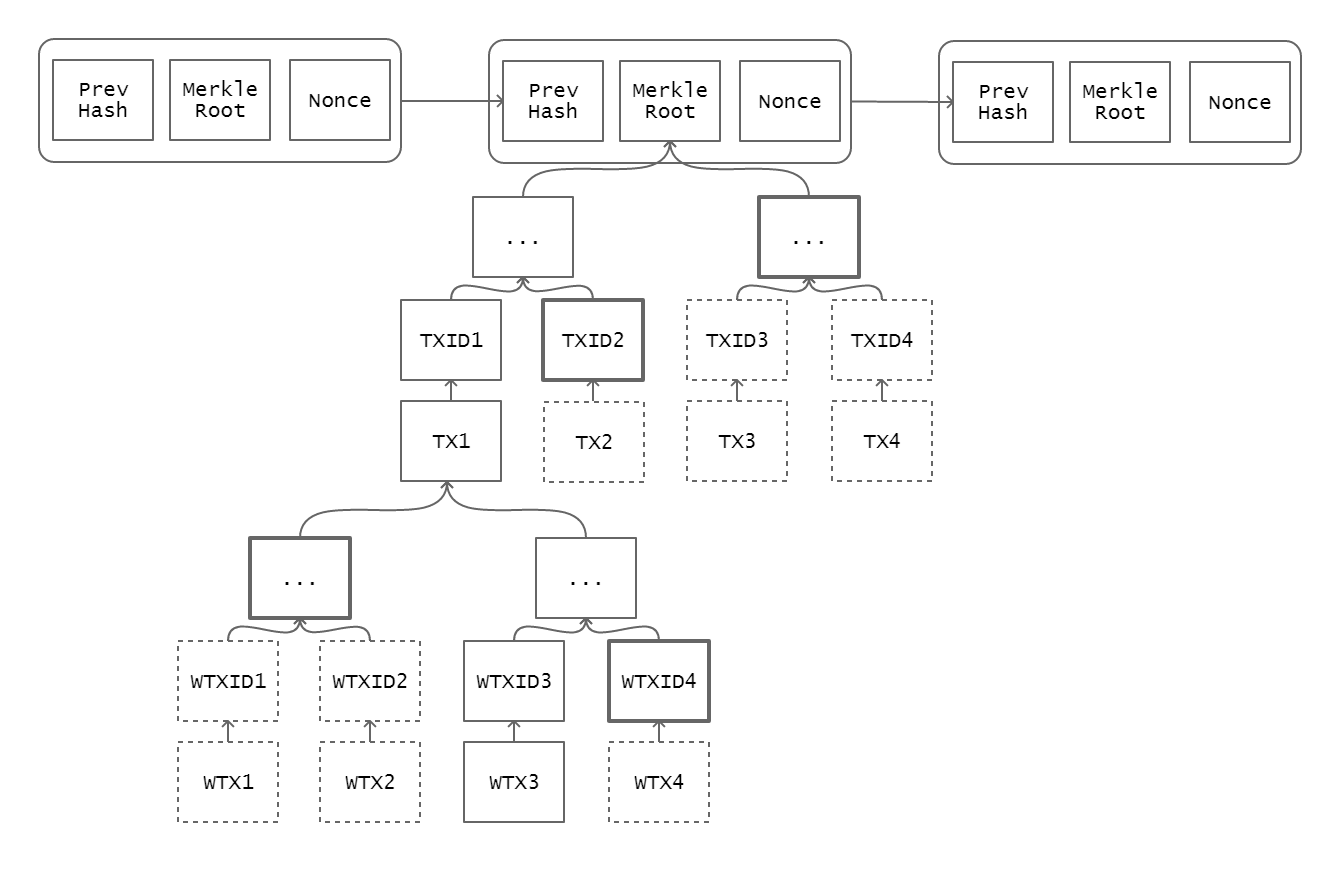
\includegraphics[width=\linewidth]{Images/bitcoin-chain-s2c-segwit.png}
		\caption[\textit{sign-to-contract} with segwit.]{\textit{sign-to-contract} with segwit. The signature is in the transaction with the witness $WTX_3$, which is committed to the coinbase $TX_1$, which is committed to Merkle root.}
		\label{fig:s2c-segwit}
	\end{center}
\end{figure} 


\section{\textit{sign-to-contract} Made Accessible}
The \textit{sign-to-contract} technique can be integrated in every Bitcoin singing software, so that, completely for free, it will also create timestamps.
To make this accessible to everyone we developed a plugin for a popular open source wallet: Electrum \cite{ElectrumWeb} \cite{ElectrumGithub}. 
Electrum is a lightweight wallet, is similar to Simple Payment Verification (SPV) wallets, but instead it asks information to special nodes called the Electrum servers. The wallet, written in python, has very few requirements despite being really flexible, of course it comes at a price: privacy and security are not at the highest standard, unless it is used in very specific ways\footnote{Offline signing and connecting to a personal Electrum server would provide a satisfying but expensive solution.}.
Having said this, it is completely functional for many purposes and it lends itself to host plugins that extend its working, like hardware wallet signing. 
Its features lead our choice to Electrum.

To run Electrum with the plugin it is necessary to use the library python-opentimestamps including \verb|OpSecp256k1Commitment| and to include the plugin among the electrum source files. All the detailed instruction, along with the files constituting the plugin, can be found at \url{https://github.com/LeoComandini/electrum-timestamp-plugin} currently in the experimental branch \textit{s2c}\footnote{The guide to install and run this specific version of the plugin is README-S2C.md and can be found in the experimental branch. For this work refer to commit aef2ee25, in the future we hope to improve the code.}. The reason behind this complicated workaround is that, at this phase, the code is intended for developers for testing purposes, not yet for a general public.

If one is familiar with Electrum code, and if the whole framework of \textit{sing-to-contract} is clear, the implementation is pretty straightforward.  We tried to be the less invasive as possible by using the hooks already present in the code and to keep, this, combined with the deliberate choice to make the code the simplest possible, lead to a suboptimal user experience. 
The signature procedure mimic the standard one adopted by Electrum, the incomplete timestamp and the data necessary to create timestamps is stored in a json file to facilitate debug.
Moreover we do not manage \textit{sign-to-contract} with segwit, since Electrum servers do not support an RPC to retrieve the Merkle path from a transaction with the witness to the coinbase and then to the block header Merkle root.

In Figure \ref{fig:enable-plugin}, \ref{fig:s2c}, \ref{fig:tx-history} and \ref{fig:upgrade} we display few screenshot to give a taste of what the plugin look like.

\begin{figure}
	\begin{center}
		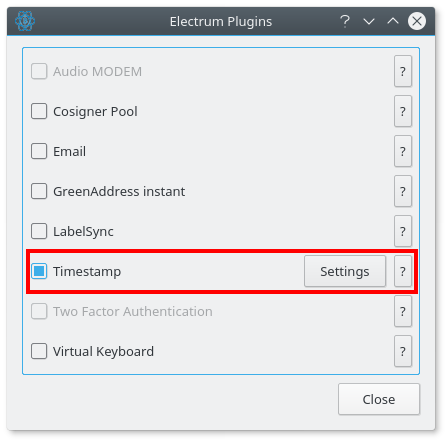
\includegraphics[width=0.5\linewidth]{Images/enable-plugin.png}
		\caption[Enable the plugin to create timestamps.]{Enable the plugin to create timestamps. This will let you select files and create OpenTimestamps proof for them.}
		\label{fig:enable-plugin}
	\end{center}
\end{figure} 

\begin{figure}
	\begin{center}
		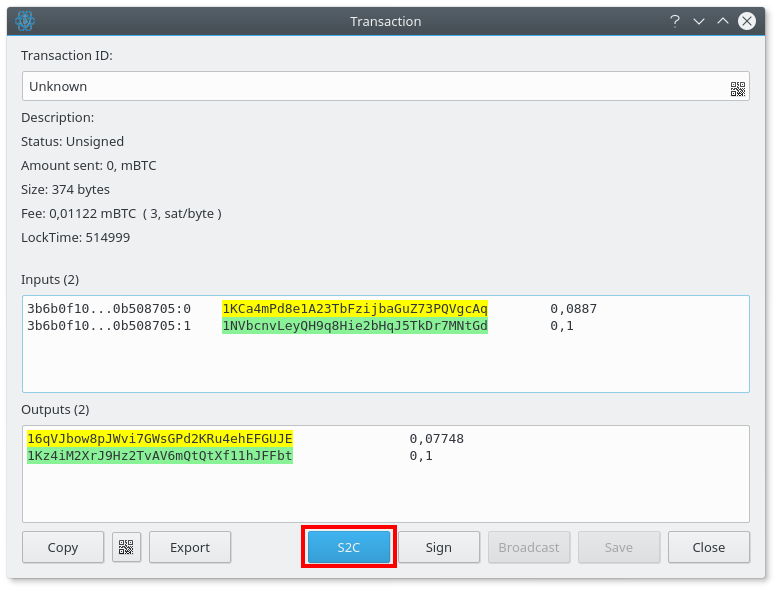
\includegraphics[width=0.9\linewidth]{Images/s2c.png}
		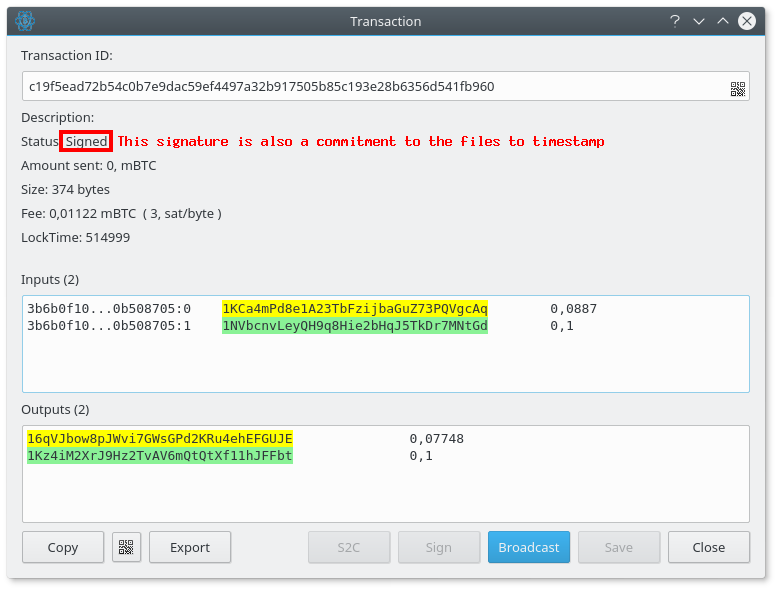
\includegraphics[width=0.9\linewidth]{Images/s2c-done.png}
		\caption[Sign with \textit{sign-to-contract}.]{Sign with \textit{sign-to-contract}. Sign and create a commitment clicking S2C then broadcast the transaction to the network.}
		\label{fig:s2c}
	\end{center}
\end{figure} 

\begin{figure}
	\begin{center}
		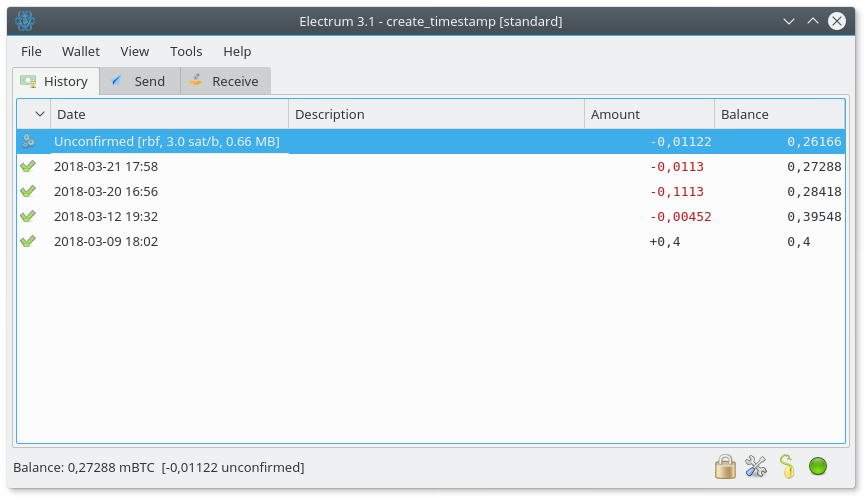
\includegraphics[width=\linewidth]{Images/tx-history.png}
		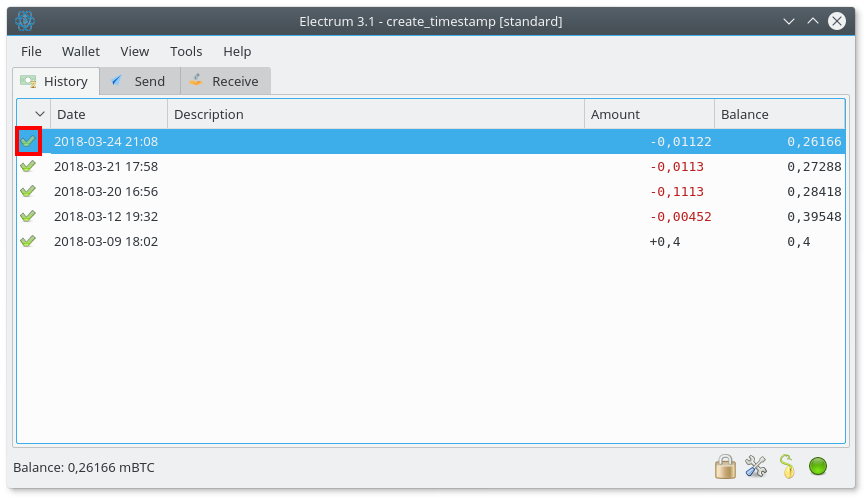
\includegraphics[width=\linewidth]{Images/tx-history-confirmed.png}
		\caption[Transaction history.]{Transaction history. Wait until the transaction is confirmed.}
		\label{fig:tx-history}
	\end{center}
\end{figure} 

\begin{figure}
	\begin{center}
		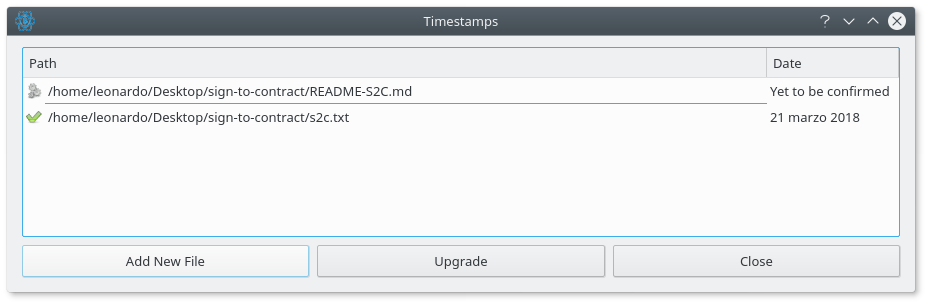
\includegraphics[width=\linewidth]{Images/pending-attestation.png}
		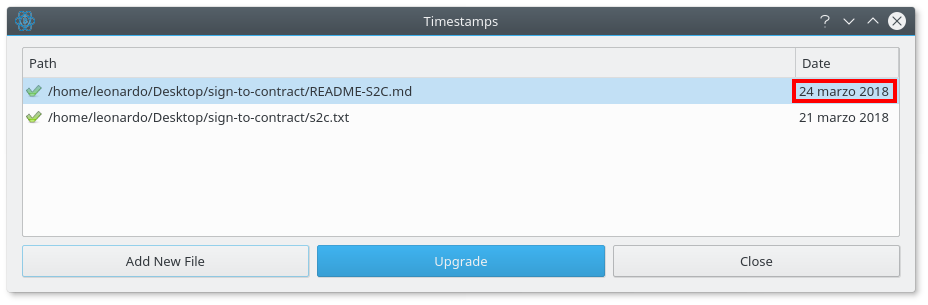
\includegraphics[width=\linewidth]{Images/post-upgrade.png}
		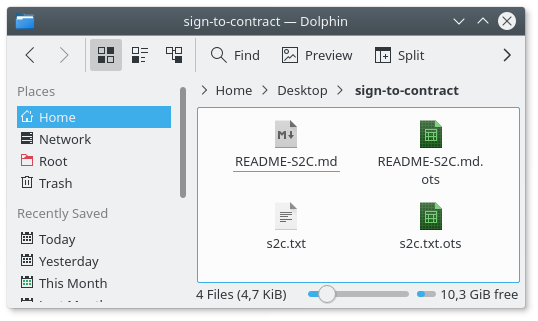
\includegraphics[width=0.7\linewidth]{Images/file-and-ots.png}
		\caption[Complete the timestamp.]{Complete the timestamp. Click on upgrade to terminate the timestamp construction. Then the proof is placed next to the timestamped file.}
		\label{fig:upgrade}
	\end{center}
\end{figure} 


At this stage, where  the \verb|OpSecp256k1Commitment| is not yet part of the standard OpenTimestamps library, the plugin may help testing the timestamping with elliptic curve commitments. 
If and when the improvement proposal will be merged, after in-depth testing has been passed, we may ask to include the plugin in the standard release of Electrum.

\chapter{Conclusions and Future Work}
\label{chpr:conclusions}
Trustless timestamping represents the highest level of security for a timestamp. 
Bitcoin and similar systems make it possible.
OpenTimestamps solves the problem of defining a common standard protocol: its public calendars fix the scalability issue allowing anyone to timestamp for free with minimal and temporary trust requirements.
Elliptic curve commitments can improve OpenTimestamps by giving the possibility to timestamp at zero marginal cost. 
If confined to Bitcoin, they give rise to two practical techniques: \textit{pay-to-contract} if the commitment is done using the payee public key, \textit{sign-to-contract} if the commitment is included in the signature. 
The first is viable but leads the user out of a BIP32 logic and this may compromise his funds in case of unexpected malfunctioning; the second does not involve this kind of risk, hence it should be preferred. 
Thanks to our integration with the bitcoin wallet Electrum, \textit{sign-to-contract} can be tested and it is easily accessible.

To push this work further, the next step should be the inclusion of \verb|OpSecp256k1Commitment| in the python-opentimestamp library.
However, with segwit, proofs double in size and it is harder to retrieve the information to independently create the timestamps: this is a problem that would deserve some research, to assess if it could be addressed in some way.

Further research could then go in different directions.
One path would be the definition of a reasonable set of rules to allow simple users to help the calendar by performing external timestamping when signing their own transactions.
Another one could consist in improving the Electrum experience, by adding a RPC to the Electrum server to retrieve the WTXID Merkle tree so to independently complete \textit{sing-to-contract} proofs or by embedding the possibility to cooperate with calendars providing external timestamps.
Deeper study of elliptic curve commitments to examine applications beyond timestamping \cite{TapRoot} is also a promising avenue for research.


%----------------------------------------------------------------------------------------
%	THESIS CONTENT - APPENDICES
%----------------------------------------------------------------------------------------

\appendix
\chapter{From Abstract Algebra to Finite Fields}
\label{app:A}
% handbook of applied cryptography

In this section we recall the formal definitions from \cite{Menezes97handbookof} to properly understand what a finite field is.

\section{Groups}
\begin{mydef} A binary operation $*$ on a set $S$ is a mapping  $S \times S$ to $S$. That is, $*$ is a rule which assigns to each ordered pair of elements from $S$ an element of $S$. \end{mydef}

\begin{mydef} 
	A group $(G, *)$ consists of a set $G$ with a binary operation $*$ on G satisfying
	the following three axioms.
	\begin{itemize}
		\item[(i)] The group operation is associative. That is, $a* (b * c) = (a* b) * c \quad \forall a, b, c \in G$.
		\item[(ii)] There is an element $1 \in G$, called the identity element, such that $a * 1 = 1 * a = a \quad \forall a \in G$.
		\item[(iii)] For each $a \in G $ there exists an element $a^{-1} \in G$, called the inverse of $a$, such that $a *a^{-1}= a^{-1} * a = 1$.
	\end{itemize}
	A group G is Abelian (or commutative) if, furthermore,
	\begin{itemize}
		\item[(iv)] $a * b = b * a \quad \forall a, b \in G$. 
	\end{itemize}
\end{mydef}

\begin{mydef} 
	A group $G$ is finite if $|G|$ is finite. The number of elements in a finite group is called its order.
\end{mydef}

\begin{myexample} 
	The set of integers $\mathbb{Z}$ with the operation of addition forms a group. 
	The identity element is 0 and the inverse of an integer $a$ is the integer $−a$. \end{myexample}

\begin{myexample} 
	The set $\mathbb{Z}_n$, with the operation of addition modulo $n$, forms a group of order $n$. 
	The set $\mathbb{Z}_n$ with the operation of multiplication modulo $n$ is not a group, since not all elements have multiplicative inverses. 
\end{myexample}

\begin{mydef} 
	The multiplicative group of $\mathbb{Z}_n$ is $\mathbb{Z}_n^* = \{a \in \mathbb{Z}_n | gcd(a, n) = 1\}$. 
	In particular, if n is a prime, then $\mathbb{Z}_n^* = \{a | 1 \leq a \leq n − 1\}$.
\end{mydef}

\begin{myexample} 
	The set $\mathbb{Z}_n^*$ is a group under the operation of multiplication modulo $n$, with identity element 1.\end{myexample}

\begin{mydef}
	A non-empty subset $H$ of a group $G$ is a subgroup of $G$ if $H$ is itself a group
	with respect to the operation of $G$. If $H$ is a subgroup of $G$ and $H \neq G$, then $H$ is called a proper subgroup of $G$.
\end{mydef}

\begin{mydef} 
	A group $G$ is cyclic if there is an element $α \in G $such that for each $b \in G$ there is an integer $i$ with $b= \alpha^i$. Such an element $\alpha$ is called a generator of $G$. 
\end{mydef}

\section{Rings}

\begin{mydef} 
	A ring $(R,+,\times)$ consists of a set $R$ with two binary operations arbitrarily denoted $+$ (addition) and $\times$ (multiplication) on $R$, satisfying the following axioms.
	\begin{itemize}
		\item[(i)] $(R, +)$ is an abelian group with identity denoted $0$.
		\item[(ii)] The operation $\times$ is associative. That is, $a \times (b \times c) = (a \times b)\times c \quad \forall a, b, c \in R$.
		\item[(iii)] There is a multiplicative identity denoted $1$, with $1 \neq 0$, such that $1 \times a = a \times 1 = a \forall a \in R.$.
		\item[(iv)] The operation $\times$ is distributive over $+$. That is, $a \times (b+c) = (a \times b)+(a \times c) \textmd{ and } (b + c) \times a = (b \times a) + (c \times a) \quad \forall a, b, c \in R.$
		
	\end{itemize} 
	The ring is a commutative ring if $a \times b = b \times a \quad \forall a, b \in R$.
\end{mydef}

\begin{myexample}
	The set $\mathbb{Z}_n$ with addition and multiplication performed modulo $n$ is a commutative ring.
\end{myexample}

\begin{mydef} 
	An element $a$ of a ring $R$ is called a unit or an invertible element if there is an element $b \in R $ such that $a \times b = 1$. 
	The set of units in a ring $R$ forms a group under multiplication, called the group of units of $R$.
\end{mydef}

\begin{myexample} 
	The group of units of the ring $\mathbb{Z}_n$ is $\mathbb{Z}_n^*$. 
\end{myexample}


\section{Fields}

\begin{mydef} 
	A field is a commutative ring in which all non-zero elements have multiplicative inverses.  
\end{mydef}

\begin{myexample} 
	the rational numbers $\mathbb{Q}$, the real numbers $\mathbb{R}$, and the complex numbers $\mathbb{C}$ form fields of characteristic $0$ under the usual operations. 
\end{myexample}

\begin{mydef} 
	The characteristic of a field is 0 if $\overbrace{1+1+\dots+1}^{m times}$ is never equal to $0$ for any $m \geq 1$. Otherwise, the characteristic of the field is the least positive integer $m$ such that $\sum_{i=1}^{m}1 = 0$.
\end{mydef}

\begin{myexample} 
	$\mathbb{Z}_n$ is a field (under the usual operations of addition and multiplication modulo $n$) if and only if $n$ is a prime number. If $n$ is prime, then $\mathbb{Z}_n$ has characteristic $n$. 
\end{myexample}

\section{Finite Fields}

\begin{mydef} 
	A finite field is a field $F$ which contains a finite number of elements. The order of $F$ is the number of elements in $F$. \end{mydef}

\begin{myprop}
	(existence and uniqueness of finite fields)
	\begin{itemize}
		\item[(i)] If $F$ is a finite field, then $F$ contains $p^m$ elements for some prime $p$ and integer $m \geq 1$.
		\item[(ii)] For every prime power order $p^m$, there is a unique (up to isomorphism) finite field of order $p^m$. This field is denoted by $\mathbb{F}_{p^m}$, or sometimes by $GF(p^m)$\footnote{Galois Field}.
	\end{itemize}
	Informally speaking, two fields are isomorphic if they are structurally the same, although the representation of their field elements may be different. Note that if $p$ is a prime then $\mathbb{Z}_p$ is a field, and hence every field of order $p$ is isomorphic to $\mathbb{Z}_p$. Thus the finite field $\mathbb{F}_p$ can be identified with $\mathbb{Z}_p$.
\end{myprop}

\chapter{Plugin functioning}
\label{app:B}
In this Appendix we outline how the plugin works to highlight how \textit{sign-to-contract} was integrated.
We aim to give an overview on which are the difficulties that arise when integrating this scheme in a signing software, while avoiding to focus on the complications related to where we decided to set our implementation.
Note that although \textit{sign-to-contract} per se is not extremely complicated, the workaround to use it to timestamp involves actions related to very disparate contexts: hashing the file, communicate with network, create a bitcoin transaction, extract the key from the wallet, perform elliptic curve math, properly encode the signature and then the transaction, broadcast the transaction, retrieve the information to complete the proof and finally correctly serialize the timestamp.
Explaining in details how all those actions are performed goes beyond the purpose of this work, for a deeper analysis, examine the code. We proceed by illustrating the plugin functioning, use Figure \ref{fig:plugin-scheme} to follow the description. 

The procedure is divided in 5 steps, \verb|Add New File|, \verb|Create New TX|, \verb|S2C|, \verb|Send TX| and \verb|Upgrade|. 
When running the application, each of these steps needs some action to be performed and a button to be pressed, in this sense they pause the flow of the procedure.

At first stage, it is possible to add new files to timestamp. 
They are included in a support database: it is stored their path and the corresponding incomplete proof, which, at this phase, is the file hash. 
In the following steps, the proof is extended with the new operations that are applied to the hash value.

The second phase consists in creating a new transaction. 
Once chosen the destination for the coins, it is performed a coin selection among the UTXOs in the wallet, the result is an unsigned transaction $uTX$. 

Then one may sign $uTX$ in the standard way, by pressing \verb|sign|, or with \textit{sign-to-contract}, pressing \verb|S2C|. 
If the latter is chosen, all the files to timestamp in the database are salted and then committed in a Merkle tree, with tip $MT$.
The operations of each branch are appended to the corresponding proof, as a result all the proofs lead to $MT$.
Then the actual \textit{sign-to-contract} procedure is implemented, the private key is retrieved from the wallet, $uTX$ is signed with contract $MT$, generating the singed transaction $TX$.

When $TX$ is broadcast to the network, the proofs are extended until its TXID.
Then, it is necessary to wait until $TX$ is confirmed, that is when it is at least 6 blocks deep. 

Finally the upgrade phase can be performed: the Merkle path, from the TXID to the block header Merkle root, is retrieved from the network and appended to the incomplete proofs, turning them into legit timestamps.
Next to each file to timestamp is placed a \verb|.ots| file which is the serialized timestamp.

\begin{figure}
	\begin{center}
		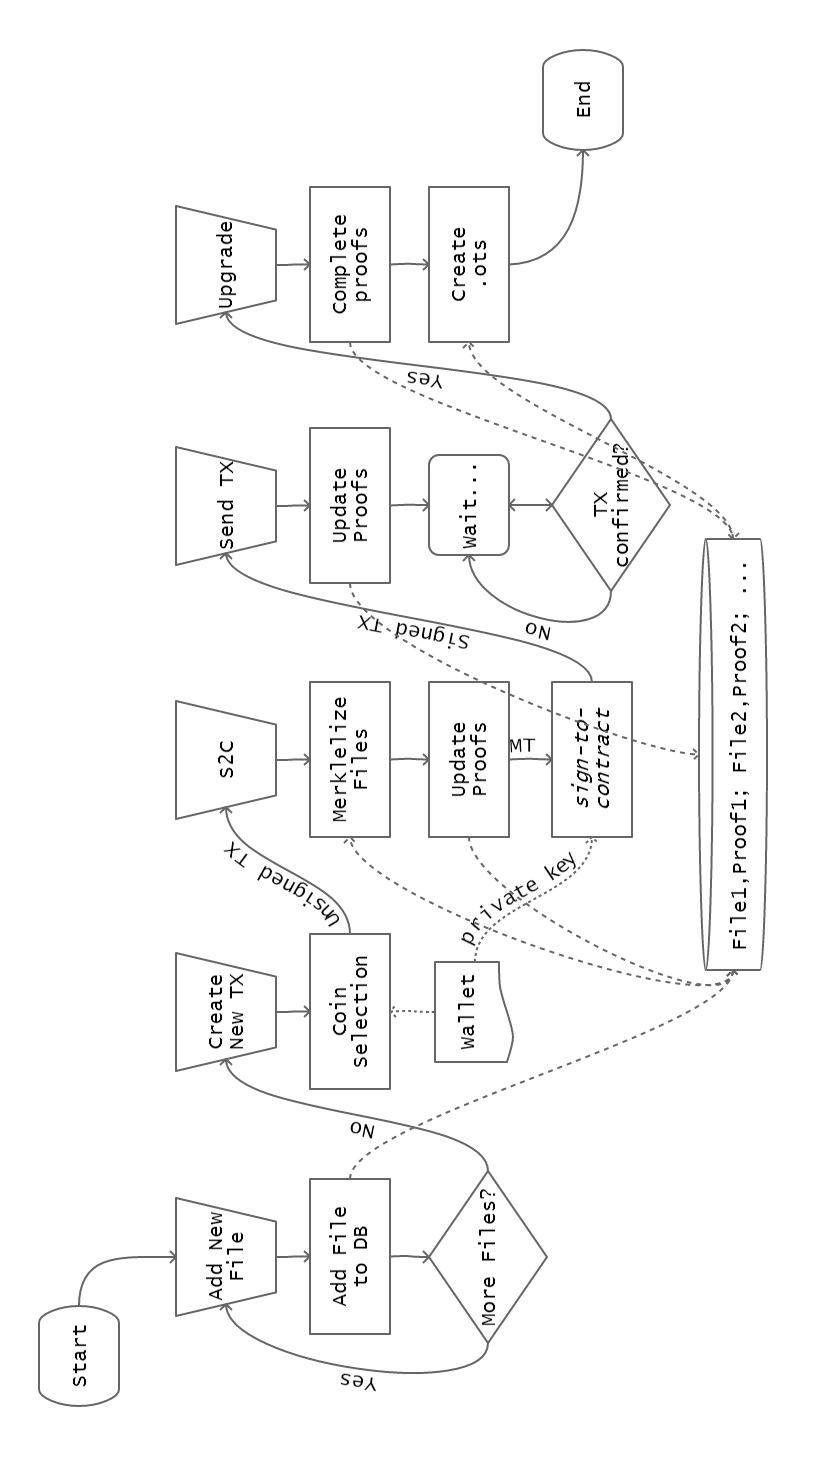
\includegraphics[width=0.75\linewidth]{Images/plugin-working.png}
		\caption[Simplified scheme of the Electrum plugin]{Simplified scheme of the Electrum plugin for \textit{sign-to-contract}.}
		\label{fig:plugin-scheme}
	\end{center}
\end{figure}


\backmatter
%----------------------------------------------------------------------------------------
%	BIBLIOGRAPHY
%----------------------------------------------------------------------------------------

\backmatter
\nocite{*}
\bibliographystyle{acm}
\bibliography{Bibliography/biblio}



\end{document}  